\documentclass[12pt]{article}
\usepackage[utf8]{inputenc}
\usepackage{graphicx}
\usepackage{float}
\usepackage[left=2.5cm,right=2cm,top=2cm,bottom=2cm]{geometry}
\usepackage{setspace}
\onehalfspacing
\usepackage{fancyhdr}

\pagestyle{fancy}
\fancyhf{}
\rhead{\textit{Stamurean Patrick Ioan}}
\lhead{Universitatea Politehnica Timișoara}
\chead{CTI-RO}
\rfoot{\centering{\thepage}}

\title{\uppercase{\bfseries{Sistem bazat pe AMD ZYNQ 7000 pentru validarea unui sistem de procesare de tip streaming cu interfata AXI stream}}}
\author{Candidat: Stamurean Patrick Ioan\\Coordonator științific: Profesor dr. ing. Oana Americai-Boncalo}
\date{Sesiunea: Iunie 2024}



\begin{document}
%%%%%%%%%% Titlu %%%%%%%%%%
\maketitle



%%%%%%%%%% Cuprins %%%%%%%%%%
\newpage
\renewcommand{\contentsname}{Cuprins}
\tableofcontents



%%%%%%%%%% Introducere %%%%%%%%%%
\newpage
\section{\uppercase{Introducere}}
\subsection{Obiective}

\hspace*{1cm}Obiectivul principal al acestei teze este de a proiecta și valida un sistem de procesare în flux bazat pe platforma AMD ZYNQ 7000, capabil să gestioneze eficient fluxurile de date în timp real printr-o interfață AXI Stream. Proiectul va integra funcționalități cheie în FPGA, inclusiv managementul stării (hold, soft reset), watchdog și programarea AXI Lite. În plus, software-ul încorporat pe procesorul dual-core ARM va calcula modelul C pentru blocurile de construcție a procesării în flux, în timp ce modulele DMA vor facilita intrarea și ieșirea datelor. Această lucrare va utiliza software-ul Vivado + Vitis pentru dezvoltare și va fi implementată pe hardware-ul ARM ZYNQ, urmărind un design de referință specificat\\\\
\hspace*{1cm}Obiectivele specifice includ:

\hspace*{1cm}1.Integrarea și configurarea componentelor hardware și software pe platforma AMD ZYNQ 7000.

\hspace*{1cm}2.Implementarea funcționalităților de bază și avansate în FPGA și ARM, inclusiv suport pentru întreruperi.

\subsection{Context}

\hspace*{1cm}Field-Programmable Gate Arrays (FPGA) sunt circuite integrate care pot fi configurate de utilizator după fabricare, permițând personalizarea hardware-ului pentru a satisface nevoile specifice ale aplicației. FPGA-urile sunt utilizate într-o varietate de aplicații, inclusiv procesarea semnalului, sistemele de control și calculul încorporat, datorită flexibilității, capabilităților de procesare paralelă și reconfigurabilității. Spre deosebire de microprocesoarele tradiționale, care execută instrucțiuni secvențial, FPGA-urile pot efectua mai multe operații simultan, ceea ce duce la îmbunătățiri semnificative ale performanței în aplicațiile adecvate.\\\\
\hspace*{1cm}Familia Zynq-7000 de la AMD combină flexibilitatea unui FPGA cu puterea de procesare a unui procesor dual-core ARM Cortex-A9. Această arhitectură face parte din familia Zynq-7000 All Programable SoC (System on Chip), care integrează atât logica programabilă, cât și sistemele de procesare pe un singur cip. Această combinație oferă o platformă versatilă pentru dezvoltarea sistemelor complexe, de înaltă performanță, care pot fi adaptate pentru sarcini specifice, făcându-l ideal pentru aplicații în sistemele auto, industriale și de comunicații.\\\\\\\\\\
\hspace*{1cm}Proiectarea și validarea unui sistem de procesare în flux bazat pe platforma AMD ZYNQ 7000 reprezintă o provocare tehnologică semnificativă datorită complexității și cerințelor de performanță impuse de aplicațiile moderne. Sistemele de procesare în flux sunt esențiale pentru gestionarea eficientă a fluxurilor de date în timp real, utilizate în diverse domenii, cum ar fi telecomunicațiile, procesarea video și analiza datelor, oferind o soluție flexibilă și de înaltă performanță pentru implementarea aplicațiilor de procesare a datelor în timp real. Utilizarea unei interfețe AXI Stream permite transferul rapid de date între diferitele componente ale sistemului, asigurând un randament ridicat și o latență scăzută.

\subsection{Prezentare generală a FPGA-urilor și arhitecturii Zynq-7000}

\hspace*{1cm}\textbf{Vivado Design Suite} și \textbf{Vitis Unified Software Platform} sunt instrumentele principale furnizate de AMD pentru dezvoltarea FPGA și SoC. Vivado este o suită cuprinzătoare pentru design hardware, care oferă instrumente avansate de sinteză și analiză, integrator IP (proprietate intelectuală) și capabilități de simulare. Le permite designerilor să dezvolte și să optimizeze design-uri FPGA cu eficiență și precizie ridicate.\\\\
\hspace*{1cm}\textbf{Vitis}, pe de altă parte, este un mediu de dezvoltare software conceput pentru procesoarele încorporate AMD, permițând dezvoltatorilor să programeze procesoarele ARM și logica programabilă într-o manieră unificată. Acceptă o gamă largă de modele de programare, de la C/C++ de nivel înalt și OpenCL până la limbaje de descriere hardware de nivel scăzut. Integrarea Vivado și Vitis permite un flux de lucru fără întreruperi în care accelerarea hardware poate fi gestionată eficient împreună cu dezvoltarea de software, asigurând performanța optimă a sistemului final.

\subsection{Context istoric și tendințe actuale}

\hspace*{1cm}\textbf{Historical Context}. \textbf{Field-Programmable Gate Arrays (FPGA)} au fost introduse în anii 1980 de către Xilinx ca o alternativă flexibilă la circuitele integrate specifice aplicației (ASIC), care sunt costisitoare și necesită timp pentru proiectare și fabricare. Primul FPGA a constat dintr-o matrice de blocuri logice configurabile (CLB) conectate prin interconexiuni programabile, permițând utilizatorilor să configureze hardware-ul în funcție de nevoile lor specifice după fabricație.\\\\
\hspace*{1cm}În anii 1960, introducerea MOSFET-urilor (tranzistoare cu efect de câmp metal-oxid-semiconductor) a marcat o piatră de hotar semnificativă în dezvoltarea FPGA. Acești tranzistori sunt componente fundamentale ale FPGA-urilor, acționând ca comutatoare electronice care pot fi pornite sau oprite pe baza semnalelor de intrare. Această tehnologie a pus bazele dispozitivelor logice programabile care vor evolua în FPGA-uri moderne.\\
\hspace*{1cm}\textbf{Tendințe curente}. Astăzi, FPGA-urile sunt utilizate într-o gamă largă de aplicații datorită performanței și flexibilității lor ridicate. Ele sunt cruciale în industrii precum telecomunicațiile, autovehiculele, aerospațiale și medicale. Progresele în tehnologia FPGA au condus la un consum redus de energie și la creșterea performanței prin tehnici precum scalarea dinamică a tensiunii și clock gating. Instrumentele de sinteză la nivel înalt (HLS) permit dezvoltatorilor să programeze FPGA-uri folosind limbaje de nivel înalt precum C/C++, simplificând procesul de dezvoltare și accelerând timpul de lansare pe piață.

\subsection{Plan de executie Milestone-uri}
\textbf{Săptămâna 1: Inițierea proiectului}\\
Task 1.1: Efectuați o revizuire detaliată a cerințelor și specificațiilor proiectului.\\
Task 1.2: Configurați mediul de dezvoltare: Instalați Vivado+EDK și pregătiți configurarea hardware-ului ARM ZYNQ.\\
Task 1.3: Elaborarea planului inițial al proiectului, inclusiv etapele de referință și livrabile.\\\\
\textbf{Săptămâna 2: Proiectare și planificare preliminară}\\
Task 2.1: Aprofundare în documentația AMD ZYNQ 7000 și în nucleele IP relevante (SISTEMUL DE PROCESARE ZYNQ, BRAM, FIFO etc.).\\\\
\textbf{Săptămâna 3: Dezvoltarea funcționalității de bază FPGA - Partea 1}\\
Task 3.1: Începeți dezvoltarea FPGA cu funcționalități de bază: hold, soft reset și timestamp.\\
Task 3.2: Implementați funcționalitatea watchdog și interfața de bază de programare AXI Lite.\\
Task 3.3: Efectuați testarea inițială a funcționalităților FPGA implementate.\\\\
\textbf{Săptămâna 4: Dezvoltarea funcționalității de bază FPGA - Partea 2}\\
Task 4.1: Dezvoltați FIFO de intrare și FIFO de ieșire pentru fluxul de date.\\
Task 4.2: Efectuați testarea inițială a funcționalităților FPGA implementate.\\\\
\textbf{Săptămâna 5: Configurare DMA și integrare software}\\
Task 5.1: Configurați DMA pentru fluxul de intrare și de ieșire.\\
Task 5.2: Începeți integrarea funcționalităților FPGA cu software-ul încorporat.\\\\
\textbf{Săptămâna 6: Integrarea sistemului și testarea inițială}\\
Task 6.1: Integrați toate funcționalitățile FPGA dezvoltate.\\
Task 6.2: Efectuați testarea integrării la nivel de sistem.\\\\\\
\textbf{Săptămâna 7 - 8 - 9 - 10: Dezvoltare software încorporat - Configurare inițială}\\
Task 7/ 8/ 9/ 10.1: Mediul de dezvoltare a procesorului dual-core ARM.\\
Task 7/ 8/ 9/ 10.2: Dezvoltarea modelului C pentru blocurile de procesare în flux.\\
Task 7/ 8/ 9/ 10.3: Multithreading de bază și gestionarea întreruperilor în software.\\\\
\textbf{Săptămâna 11: Dezvoltare și optimizare avansată de software}\\
Task 11.1: Optimizați software-ul încorporat pentru performanță și fiabilitate.\\
Task 11.2: Îmbunătățiți software-ul cu funcții suplimentare bazate pe feedback-ul de testare a integrării.\\
Task 11.3: Implementați capabilități avansate de gestionare a întreruperilor și multithreading.\\\\
\textbf{Săptămâna 12: Testare cuprinzătoare a sistemului}\\
Task 12.1: Efectuați teste cuprinzătoare ale sistemului, inclusiv teste de stres, performanță și fiabilitate.\\
Task 12.2: Rafinați sistemul pe baza rezultatelor cuprinzătoare ale testării.\\
Task 12.3: Validați funcționalitatea finală a sistemului în raport cu cerințele inițiale.\\\\
\textbf{Săptămâna 13 - 14 - 15: Finalizare și documentare}\\
Task 13/ 14/ 15.1: Finalizați toate funcționalitățile sistemului și asigurați conformitatea cu specificațiile proiectului.\\
Task 13/ 14/ 15.2: Compilați documentația cuprinzătoare a proiectului, inclusiv detalii de proiectare, cod, proceduri de testare și rezultate.\\
Task 13/ 14/ 15.3: Pregătiți un manual de utilizare sau un ghid pentru sistemul dezvoltat.\\\\
\textbf{Săptămâna 16: Închiderea și prezentarea proiectului}\\
Task 16.1: Pregătiți prezentarea finală a proiectului, concentrându-se pe obiective, proces, provocări, soluții și realizări.\\
Task 16.2: Repetați prezentarea și anticipați întrebările.\\
Task 16.3: Trimiteți toate livrabilele proiectului, inclusiv codul, documentația și materialele de prezentare.\\
Task 16.4: Prezentați proiectul.\\\\

\begin{figure}[ht]
\centering
%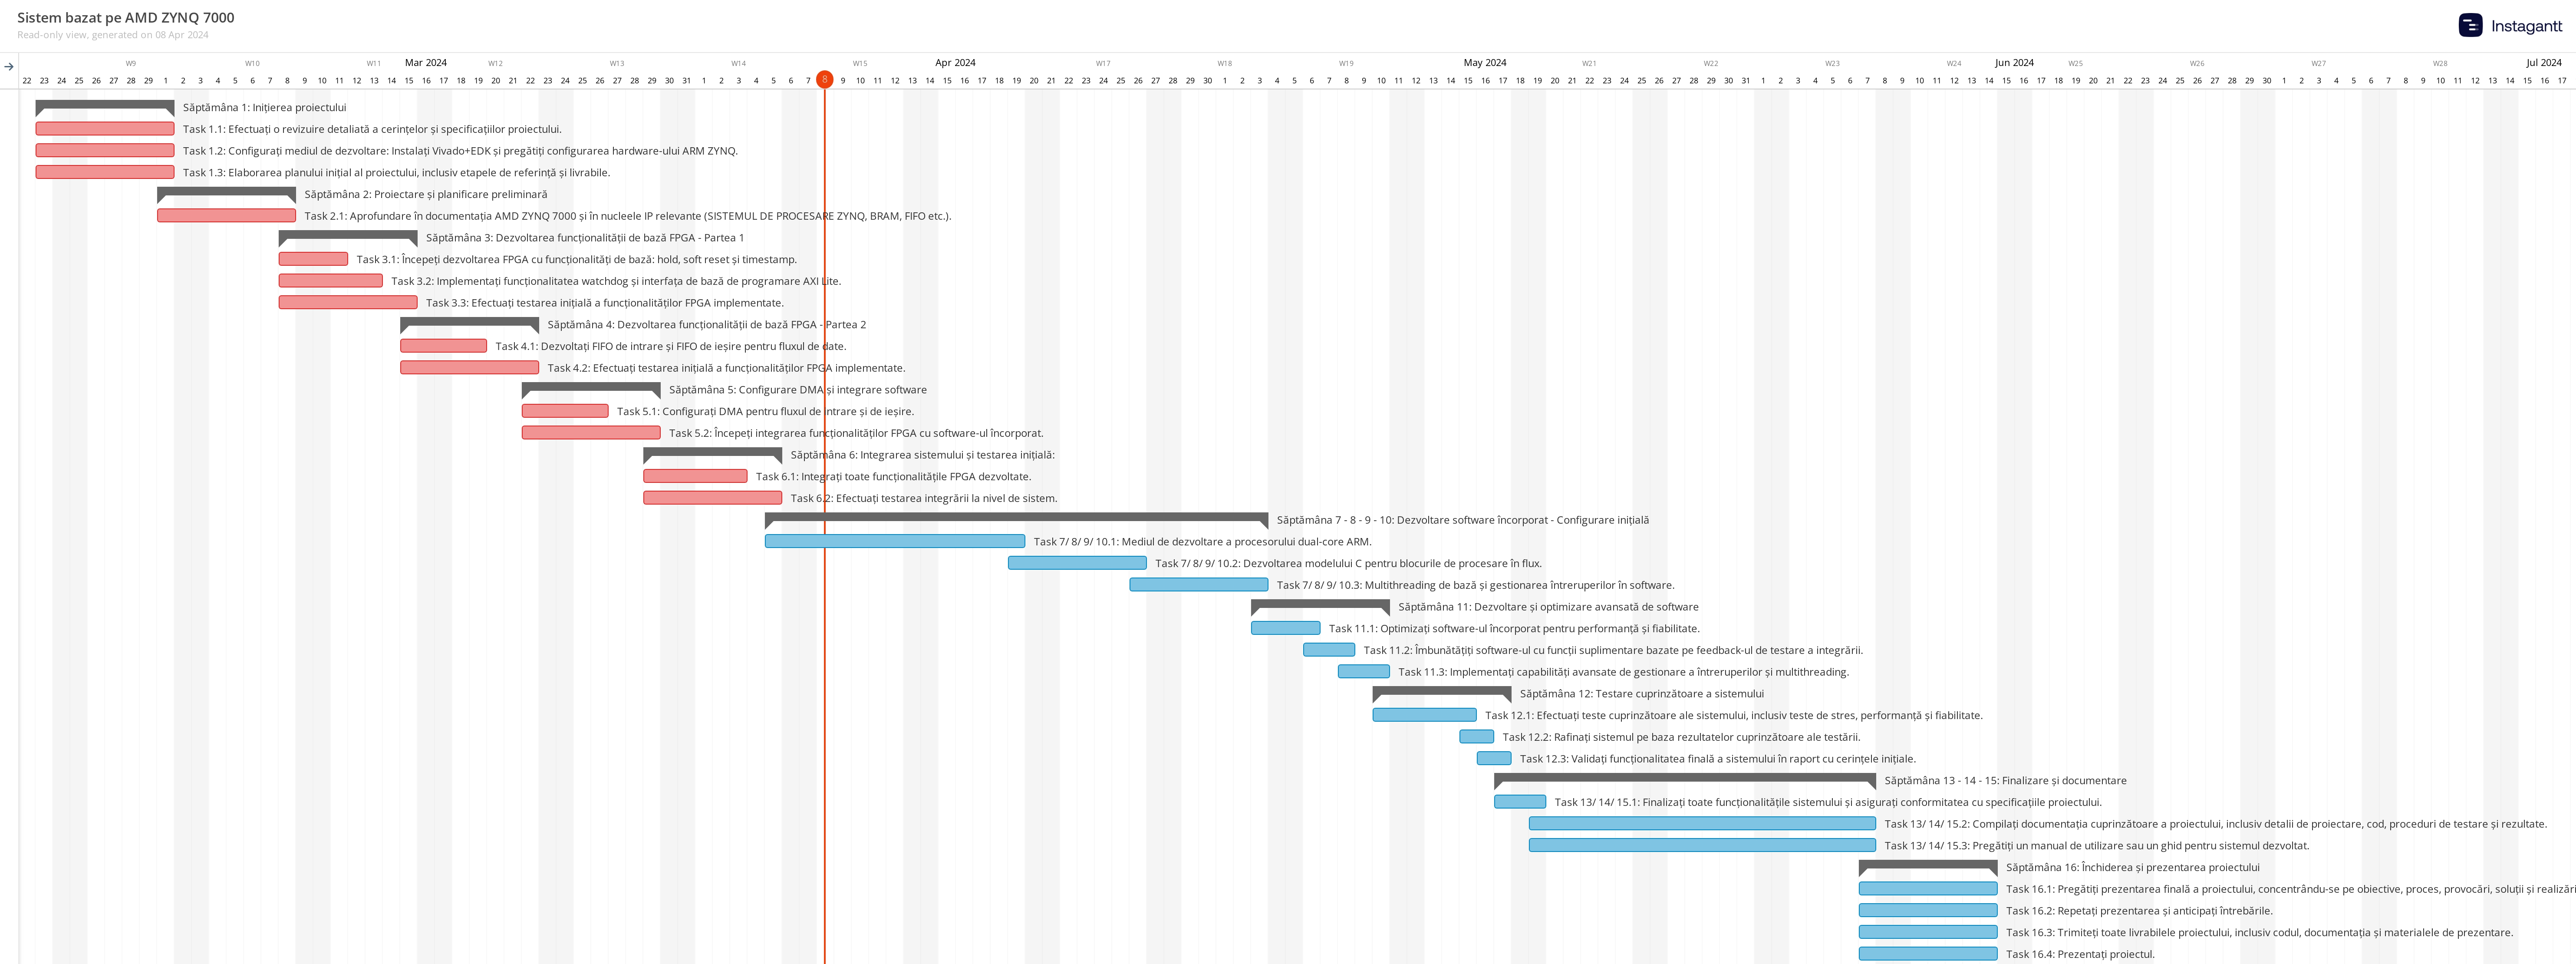
\includegraphics[width=1\textwidth]{../Licenta_Stamurean_Patrick_Ioan/Milestones.jpg}
\caption{Milestones Gantt Chart \textbf{[1]}}
\end{figure}



%%%%%%%%%% Metodologii %%%%%%%%%%
\newpage
\section{\uppercase{Metodologii}}
\subsection{Configurare hardware: Descrierea Zynq-7000 ZedBoard și a dispozitivelor periferice}

\subsubsection{Zynq-7000 ZedBoard Prezentare generală}

\hspace*{1cm}ZedBoard este o placă de dezvoltare și evaluare bazată pe Xilinx Zynq-7000 All Programable System-on-Chip (SoC). Această platformă inovatoare integrează un procesor ARM Cortex-A9 dual-core cu logică programabilă (PL) bazată pe tehnologia FPGA din seria 7 de la Xilinx, oferind o soluție puternică și flexibilă pentru o gamă largă de aplicații.

\subsubsection{Caracteristici și specificații cheie}

\textbf{Caracteristici și specificații}


\begin{itemize}
    \item \textbf{Procesor și FPGA:}
    \begin{itemize}
        \item \textbf{Procesor:} Dual-core ARM Cortex-A9
        \item \textbf{FPGA:} XC7Z020-1CSG484 (Zynq-7000 AP SoC)
    \end{itemize}
    \item \textbf{Memorie:}
    \begin{itemize}
        \item 512 MB DDR3 RAM
        \item 256 MB QSPI Flash
    \end{itemize}
    \item \textbf{Interfete:}
    \begin{itemize}
        \item Programare USB-JTAG
        \item 10/100/1G Ethernet
        \item USB OTG 2.0
        \item SD Card slot
        \item USB-UART bridge
        \item HDMI and VGA outputs
        \item 128x32 Display OLED
        \item Audio (line-in, line-out, headphone, mic)\\\\\\
    \end{itemize}
    \item \textbf{Conectivitate:}
    \begin{itemize}
        \item 5 conectori Pmod (unul pentru PS (Processing System), 4 pentru PL(Programable Logic))
        \item 1 LPC FMC connector
        \item 1 AMS header
    \end{itemize}
    \item \textbf{Interfata cu utilizatorul:}
    \begin{itemize}
        \item 2 butoane reset (unul pentru PS, unul pentru PL)
        \item 7 butoane
        \item 8 comutatoare DIP
        \item 9 LED-uri de utilizator (1 pentru PS, 8 pentru PL)
        \item LED DONE care indică starea configurației FPGA\\
    \end{itemize}
\end{itemize}


\noindent \textbf{Dispozitive periferice}
\begin{enumerate}
    \item \textbf{Conectori Pmod:} ZedBoard include cinci conectori Pmod care oferă acces la I/O logic programabil. Acești conectori pot fi utilizați pentru interfața cu diverse module periferice (Pmods) pentru extinderea funcționalității plăcii.
    \item \textbf{Porturi HDMI si VGA:} Aceste porturi permit conectarea ecranelor, permițând capabilități de ieșire video pentru aplicații precum procesarea video.
    \item \textbf{Port Ethernet:} Portul Gigabit Ethernet facilitează conexiunea la rețea, făcând ZedBoard potrivit pentru aplicații de rețea și acces la date de la distanță.
    \item \textbf{SD Card Slot:} Acceptă pornirea de pe un card SD și oferă opțiuni de stocare suplimentare pentru aplicații mai mari sau înregistrarea datelor.
    \item \textbf{Interfete Audio:} Mufele de intrare, ieșire, căști și microfon sunt disponibile pentru intrare și ieșire audio, utile în aplicațiile multimedia.
    \item \textbf{Display OLED:} Ecran OLED mic care poate fi utilizat pentru a afișa informații de stare, ieșiri sau elemente de interfață cu utilizatorul în aplicațiile încorporate.
Aplicații și cazuri de utilizare\\\\
\end{enumerate}
\hspace*{1cm}Această combinație de caracteristici și opțiuni de conectivitate face din ZedBoard o platformă ideală pentru prototipare rapidă, scopuri educaționale și dezvoltare de dovadă a conceptului pentru o gamă largă de aplicații



\subsection{Instrumente Software}

\textbf{Vivado Design Suit}\\
\hspace*{1cm}\textbf{Prezentare Generală.} Vivado Design Suite este suita completă de instrumente de la Xilinx pentru dezvoltarea designurilor FPGA și SoC. Include instrumente pentru sinteză, simulare și analiză a designurilor HDL, integrarea IP (Proprietate Intelectuală) și depanare hardware.\\\\
\hspace*{1cm}\textbf{Caracteristici Cheie}
\begin{enumerate}
    \item \textbf{Sinteză și implementare:} Transformă proiectele HDL (VHDL/Verilog) în liste de net la nivel de poartă.
    \item \textbf{IP Integrator:} facilitează integrarea blocurilor IP verificate în prealabil.
    \item \textbf{Simulator Vivado:} Oferă un mediu de simulare pentru verificarea proiectelor.
    \item \textbf{Analiză sincronizare și putere:} analizează caracteristicile de sincronizare și putere ale proiectelor.
    \item \textbf{Hardware Debugging:} Oferă instrumente pentru depanarea în timp real și validarea proiectelor pe hardware.
\end{enumerate}
\textbf{Instalare și configurare}\\\\
\textbf{Instalare pas cu pas:}\\
\begin{enumerate}
    \item \textbf{Descărcați Vivado:}
    \begin{itemize}
        \item Accesați Centrul de descărcare Xilinx.
        \item Selectați versiunea corespunzătoare a Vivado Design Suite.
        \item Descărcați programul de instalare complet pentru sistemul dvs. de operare.
    \end{itemize}
        \item \textbf{Instalați Vivado:}
    \begin{itemize}
        \item Rulați programul de instalare descărcat.
        \item Urmați instrucțiunile de pe ecran pentru a instala Vivado.
        \item Descărcați programul de instalare complet pentru sistemul dvs. de operare.
        \item Acceptați acordul de licență și finalizați instalarea.
    \end{itemize}
        \item \textbf{Configurarea Vivado:}
    \begin{itemize}
        \item Deschideți Vivado și creați un nou proiect
        \item Configurați setările proiectului.
    \end{itemize}
\end{enumerate}
\textbf{Sfaturi de configurare:}
\begin{itemize}
    \item IP Integrator: utilizați instrumentul IP Integrator pentru a adăuga și configura blocuri IP.
    \item Constrângeri: Aplicați constrângeri de sincronizare și fizice folosind fișiere XDC (Xilinx Design Constraints).
    \item Simulare: configurați mediul de simulare prin adăugarea a testbench-uri și configurarea setărilor de simulare.\\
\end{itemize}
\textbf{Vitis Unified Software Platform}\\
\hspace*{1cm}\textbf{Prezentare Generală.} Vitis este platforma software unificată a Xilinx, concepută pentru a funcționa cu hardware-ul lor (inclusiv FPGA-uri și SoC-uri). Acesta permite dezvoltatorilor să programeze atât sistemul de procesare, cât și logica programabilă.\\\\
\hspace*{1cm}\textbf{Caracteristici Cheie}
\begin{enumerate}
    \item \textbf{Dezvoltare unificată:} Combină software încorporat, biblioteci accelerate și dezvoltare de modele AI.
    \item \textbf{Sinteză la nivel înalt (HLS):} Permite compilarea codului C/C++ și OpenCL în descrierile hardware.
    \item \textbf{Aplicații versatile:} Suportă o gamă largă de aplicații, de la sisteme încorporate la acceleratoare pentru centre de date.
    \item \textbf{Integrare cu Vivado:} se integrează perfect cu Vivado pentru co-proiectare hardware/software.
\end{enumerate}
\textbf{Instalare și configurare}\\\\
\textbf{Instalare pas cu pas:}\\
\begin{enumerate}
    \item \textbf{Descărcați Vitis:}
    \begin{itemize}
        \item Vizitați Centrul de descărcare Xilinx.
        \item Selectați Vitis Unified Software Platform.
        \item Descărcați programul de instalare.
    \end{itemize}
        \item \textbf{Instalați Vitis:}
    \begin{itemize}
        \item Rulați programul de instalare Vitis.
        \item Urmați instrucțiunile de pe ecran pentru a instala Vitis.
        \item Alegeți componentele de instalare în funcție de cerințele dvs.
        \item Acceptați acordul de licență și finalizați instalarea.
    \end{itemize}
        \item \textbf{Configurarea Vitis:}
    \begin{itemize}
        \item Deschideți Vitis și configurați spațiul de lucru.
        \item Importați sau creați proiecte noi.
    \end{itemize}
\end{enumerate}
\textbf{Sfaturi de configurare:}
\begin{itemize}
    \item Configurare platformă: definiți setările platformei, inclusiv hardware-ul țintă (de exemplu, Zynq-7000).
    \item Dezvoltare de aplicații: Dezvoltați și depanați aplicații software folosind mediul de dezvoltare integrat.
    \item Accelerare hardware: Utilizați instrumentul Vitis HLS pentru a compila cod de nivel înalt în descrieri hardware compatibile cu FPGA.
\end{itemize}
\textbf{Integrarea Vivado și Vitis}\\\\
\textbf{Integrarea fluxului de lucru:}\\
\begin{enumerate}
    \item \textbf{Design hardware în Vivado:}
    \begin{itemize}
        \item Proiectați componentele hardware folosind Vivado.
        \item Exportați designul hardware, inclusiv fișierele de flux de biți și de descriere hardware.
    \end{itemize}
        \item \textbf{Dezvoltare software în Vitis:}
    \begin{itemize}
        \item Importați designul hardware în Vitis.
        \item Dezvoltați aplicații software care vizează componentele hardware.
        \item Utilizați instrumentele Vitis pentru a compila, depana și implementa aplicații.
    \end{itemize}
\end{enumerate}



\subsection{Protocoale Folosite}
\hspace*{1cm}Specificațiile AMBA AXI (Advanced eXtensible Interface) includ mai multe protocoale concepute pentru transferul rapid de date în circuite integrate, folosite în principal în designul sistemelor pe chip (SoC). Aceste protocoale sunt dezvoltate de ARM și sunt o parte esențială a arhitecturii ARM Advanced Microcontroller Bus Architecture (AMBA).\\\\
\hspace*{1cm}\textbf{AXI3} face parte din specificația AMBA 3 și introduce o metodă de comunicare bazată pe canale care îmbunătățește protocolul anterior AHB, oferind performanțe superioare, o frecvență mai mare de operare și caracteristici cum ar fi completarea tranzacțiilor în ordine neconsecutivă. Acesta este potrivit pentru transferul de date de mare viteză în designuri complexe SoC.\\\\
\hspace*{1cm}\textbf{AXI4} extinde AXI3 prin îmbunătățirea configurării lățimii interfeței și furnizarea de tranzacții burst mai eficiente. Suportă maparea de memorie de înaltă performanță și este folosit pe scară largă în aplicații care necesită un debit mare de date.\\\\
\hspace*{1cm}\textbf{AXI4-Lite} este o versiune simplificată a AXI4, proiectată pentru tranzacții mai puțin complexe, unde un debit ridicat nu este necesar. Este utilizat în mod obișnuit pentru interfețele de registru de control în cadrul SoC-urilor, datorită complexității reduse a interfeței și suprapunerii reduse de hardware.\\\\
\hspace*{1cm}\textbf{AXI4-Stream}, acest protocol este special conceput pentru datele stream. Simplifică conectivitatea prin eliminarea necesității informațiilor de adresă și control asociate fiecărui transfer de date. Este optim pentru aplicații precum transportul de date video, audio și pachete care necesită fluxuri de date continue, de mare viteză.\\



\subsection{Componente principale ale Sistemului}
\hspace*{1cm}Sistemul bazat pe AMD ZYNQ 7000 integrează o suită diversificată de blocuri de proprietate intelectuală (IP-uri) pentru a facilita procesarea eficientă și flexibilă a datelor într-un mediu de streaming. Aceste componente IP, esențiale pentru funcționalitatea și optimizarea sistemului, includ interfețe de comunicație, controlere de memorie, convertori de protocol și module de temporizare, toate configurate să lucreze împreună într-o arhitectură coerentă și robustă destinată aplicațiilor de procesare în timp real. IP-urile folosite in acest proiect, sunt: 



\subsubsection{ZYNQ 7000 Processing System (PS)}

\begin{figure}[H]
    \centering
    \includegraphics[width=0.5\textwidth]{C:/Users/patri/Desktop/Li/Latex_Poze/Zynq7000_Processing_System.png}
    \caption{Zynq7000 Processing System}
\end{figure}
 
\hspace*{1cm}Familia Zynq®-7000 se bazează pe arhitectura Xilinx All Programmable system-on-chip (AP SoC). Aceste produse integrează un sistem de procesare (PS) bazat pe ARM® Cortex™-A9 MPCore™ cu două nuclee bogate în funcții și logică programabilă Xilinx (PL) într-un singur dispozitiv, construit pe un sistem de ultimă generație, Tehnologia de proces de performanță, de putere redusă (HPL), 28 nm și cu porți metalice de înaltă k (HKMG). Procesoarele ARM Cortex-A9 MPCore sunt inima PS, care include, de asemenea, memorie pe cip, interfețe de memorie externă și un set bogat de periferice I/O. Nucleul Processing System 7 este interfața software din jurul sistemului de procesare a platformei Zynq-7000. Familia Zynq-7000 constă dintr-un PS integrat în stil SoC și o unitate PL, oferind o soluție SoC extensibilă și flexibilă pe o singură matriță. Nucleul Processing System 7 acționează ca o conexiune logică între PS și PL, în timp ce vă ajută să integrați IP-uri personalizate și încorporate cu sistemul de procesare utilizând integratorul Vivado® IP.\\\\
\hspace*{1cm}Procesor System Reset IP Core de la Xilinx este folosit pentru a gestiona și controla operațiunile de resetare a unui întreg sistem într-un FPGA. O explicație detaliată a fiecărui pin din diagrama bloc furnizată:
\begin{enumerate}
    \item \textbf{slowest\_sync\_clk:} Acest semnal de ceas de intrare este cel mai lent ceas din sistem care necesită resetare sincronizare. Acesta asigură că toate operațiunile de resetare sunt sincronizate pe diferite domenii de ceas.
    \item \textbf{ext\_reset\_in:} Această intrare este un semnal de resetare extern, adesea conectat la un buton de resetare extern sau la alte surse externe. Inițiază o resetare atunci când este afirmată, ajutând în scenariile în care un eveniment extern ar trebui să declanșeze o resetare.
    \item \textbf{aux\_reset\_in:} Această intrare auxiliară de resetare este utilizată pentru control suplimentar de resetare. Poate fi folosit pentru a iniția o resetare de la o sursă auxiliară, cum ar fi un semnal software sau o altă componentă internă.
    \item \textbf{mb\_debug\_sys\_rst:} Această intrare este utilizată de obicei pentru resetarea sistemului de depanare MicroBlaze. Se asigură că procesorul MicroBlaze și logica aferentă acestuia sunt resetate corect în timpul depanării.
    \item \textbf{dcm\_locked:} Această intrare indică starea de blocare a Digital Clock Manager (DCM). Sistemul rămâne în resetare până când DCM este blocat, asigurându-se că toate semnalele de ceas sunt stabile înainte ca sistemul să înceapă să funcționeze.
    \item \textbf{mb\_reset:} Acest semnal de ieșire resetează procesorul MicroBlaze. Este afirmat ca răspuns la intrările de resetare și este sincronizat cu ceasul sistemului.
    \item \textbf{bus\_struct\_reset[0:0]:} Acest semnal de ieșire resetează structurile magistralei din sistem. Acesta asigură că toată logica legată de magistrală este resetată și inițializată corect.
    \item \textbf{peripheral\_reset[0:0]:} Această ieșire resetează perifericele conectate la sistem. Acesta asigură că toate dispozitivele periferice pornesc dintr-o stare cunoscută după o resetare.
    \item \textbf{interconnect\_aresetn[0:0]:} Acest semnal de resetare activ-low este utilizat pentru interconexiunile AXI din cadrul sistemului. Acesta asigură resetarea și inițializarea corespunzătoare a interconexiunilor, care gestionează traficul de date între diferite componente ale sistemului.
    \item \textbf{peripheral\_aresetn[0:0]:} Acest semnal de resetare activ-low este pentru periferice, similar cu periferic\_reset, dar special conceput pentru periferice care necesită resetare activ-low.
\end{enumerate}
\hspace*{1cm}Miezul IP de resetare a sistemului procesorului este extrem de configurabil, permițându-i să se adapteze la diferite cerințe de sistem prin activarea sau dezactivarea diferitelor funcții de resetare. Acesta asigură un proces de resetare fiabil și sincronizat pentru toate componentele unui design FPGA, care este esențial pentru menținerea stabilității și a fiabilității sistemului.


\subsubsection{Processor System Reset}

\begin{figure}[H]
    \centering
    \includegraphics[width=0.5\textwidth]{C:/Users/patri/Desktop/Li/Latex_Poze/Processor_System_Reset.png}
    \caption{Processor System Reset}
\end{figure}

\hspace*{1cm}Processor System Reset este un IP soft care oferă un mecanism pentru a gestiona condițiile de resetare pentru un anumit sistem. Nucleul gestionează numeroase condiții de resetare la intrare și generează resetări corespunzătoare la ieșire. Acest nucleu generează resetările pe baza condițiilor de resetare externe sau interne.\\
Rezumatul caracteristicilor
\begin{itemize}
    \item Atât intrările de resetare externe, cât și cele auxiliare pot fi selectate ca activ-HIGH sau activ-LOW.
    \item Generare resetare la pornire. Condiția Power On Reset face ca toate ieșirile de resetare să devină active în primele două clocks ale unei porniri și să rămână active timp de 16 clocks. 
    \item Generarea semnalului de resetare activ parametrizat-scăzut pentru core și pentru interconectare.
    \item Secvențierea semnalelor de resetare care ies din resetare:
    \begin{enumerate}
        \item Structurile de autobuz ies din resetare (Interconectare și pod).
        \item Perifericele ies din resetare 16 cicluri de clock mai târziu (UART, SPI, IIC).
        \item Procesorul MicroBlaze™ iese din resetare la 16 cicluri de clock după periferice.
    \end{enumerate}
\end{itemize}
\hspace*{1cm}Procesor System Reset IP Core de la Xilinx este folosit pentru a gestiona și controla operațiunile de resetare a unui întreg sistem într-un FPGA. O explicație detaliată a fiecărui pin din diagrama bloc furnizată:
\begin{enumerate}
    \item \textbf{slowest\_sync\_clk:} acest semnal de ceas de intrare este cel mai lent ceas din sistem care necesită resetare sincronizare. Acesta asigură că toate operațiunile de resetare sunt sincronizate pe diferite domenii de ceas.
    \item \textbf{ext\_reset\_in:} Această intrare este un semnal de resetare extern, adesea conectat la un buton de resetare extern sau la alte surse externe. Inițiază o resetare atunci când este afirmată, ajutând în scenariile în care un eveniment extern ar trebui să declanșeze o resetare.
    \item \textbf{aux\_reset\_in:} Această intrare auxiliară de resetare este utilizată pentru control suplimentar de resetare. Poate fi folosit pentru a iniția o resetare de la o sursă auxiliară, cum ar fi un semnal software sau o altă componentă internă.
    \item \textbf{mb\_debug\_sys\_rst:} Această intrare este utilizată de obicei pentru resetarea sistemului de depanare MicroBlaze. Se asigură că procesorul MicroBlaze și logica aferentă acestuia sunt resetate corect în timpul depanării.
    \item \textbf{dcm\_locked}: Această intrare indică starea de blocare a Digital Clock Manager (DCM). Sistemul rămâne în resetare până când DCM este blocat, asigurându-se că toate semnalele de ceas sunt stabile înainte ca sistemul să înceapă să funcționeze.
    \item \textbf{mb\_reset:} Acest semnal de ieșire resetează procesorul MicroBlaze. Este afirmat ca răspuns la intrările de resetare și este sincronizat cu ceasul sistemului.
    \item \textbf{bus\_struct\_reset[0:0]:} Acest semnal de ieșire resetează structurile magistralei din sistem. Acesta asigură că toată logica legată de magistrală este resetată și inițializată corect.
    \item \textbf{peripheral\_reset[0:0]:} Această ieșire resetează perifericele conectate la sistem. Acesta asigură că toate dispozitivele periferice pornesc dintr-o stare cunoscută după o resetare.
    \item \textbf{interconnect\_aresetn[0:0]:} Acest semnal de resetare activ-low este utilizat pentru interconexiunile AXI din cadrul sistemului. Acesta asigură resetarea și inițializarea corespunzătoare a interconexiunilor, care gestionează traficul de date între diferitele componente ale sistemului.
    \item \textbf{peripheral\_aresetn[0:0]:} Acest semnal de resetare activ-low este pentru periferice, similar cu periferic\_reset, dar special conceput pentru periferice care necesită resetare activ-low.
\end{enumerate}
\hspace*{1cm}Miezul IP de resetare a sistemului procesorului este extrem de configurabil, permițându-i să se adapteze la diferite cerințe de sistem prin activarea sau dezactivarea diferitelor funcții de resetare. Acesta asigură un proces de resetare fiabil și sincronizat pentru toate componentele unui design FPGA, care este esențial pentru menținerea stabilității și fiabilității sistemului.



\subsubsection{AXI Interconnect} 

\begin{figure}[H]
    \centering
    \includegraphics[width=0.5\textwidth]{C:/Users/patri/Desktop/Li/Latex_Poze/AXI_Interconnect.png}
    \caption{AXI Interconnect}
\end{figure}

\hspace*{1cm}Nucleul AXI Interconnect poate fi adăugat numai la un design de bloc integrator Vivado® IP în Vivado Design Suite. Nucleul Interconnect IP reprezintă un bloc de proiectare ierarhic care conține mai multe instanțe LogiCORE™ IP (nuclee de infrastructură) care devin configurate și conectate în timpul sesiunii de proiectare a sistemului. Fiecare dintre nucleele de infrastructură poate fi, de asemenea, adăugat direct la un design bloc (în afara nucleului AXI Interconnect) sau selectat direct din Catalogul Vivado IP și configurat pentru utilizare într-un design HDL. Nucleul AXI Interconnect permite orice amestec de master AXI și dispozitivele slave care urmează să fie conectate la acesta, care pot varia între ele în ceea ce privește lățimea datelor, domeniul de clock și sub-protocolul AXI (AXI4, AXI3 sau AXI4-Lite). Când caracteristicile interfeței oricărui dispozitiv master sau slave conectat diferă de cele ale comutatorului cu bară transversală din interiorul interconexiunii, nucleele infrastructurii adecvate sunt deduse automat și conectate în cadrul interconexiunii pentru a efectua conversiile necesare.
\hspace*{1cm}Miezul AXI Interconnect IP este un modul versatil care conectează mai multe dispozitive master și slave mapate cu memorie AXI. Iată o explicație detaliată a fiecărui pin din diagrama bloc furnizată:
\begin{enumerate}
    \item \textbf{S00\_AXI:} Aceasta este interfața slave AXI primară. Acesta permite unui master AXI să inițieze tranzacții de citire și scriere la interconectare.
    \item \textbf{ACLK:} Acesta este semnalul de ceas global pentru interconectarea AXI. Sincronizează toate operațiunile din interconectare.
    \item \textbf{ARESETN:} Acesta este semnalul global de resetare activ-low. Afirmarea acestui semnal resetează întreaga interconexiune AXI.
    \item \textbf{S00\_ACLK:} Acesta este semnalul de ceas specific interfeței slave S00\_AXI. Sincronizează tranzacțiile pe această interfață specifică.
    \item \textbf{S00\_ARESETN:} Acesta este semnalul de resetare activ-scăzut pentru interfața slave S00\_AXI. Inițializează această interfață specifică atunci când este afirmată.
    \item \textbf{M00\_ACLK la M06\_ACLK:} Acestea sunt semnalele de ceas pentru fiecare interfață master respectivă (M00\_AXI la M06\_AXI). Ei sincronizează tranzacțiile pentru interfețele lor principale respective.
    \item \textbf{M00\_ARESETN la M06\_ARESETN:} Acestea sunt semnalele de resetare activ-low pentru fiecare interfață master respectivă (M00\_AXI la M06\_AXI). Ele inițializează interfețele master respective atunci când sunt afirmate.
    \item \textbf{M00\_AXI la M06\_AXI:} Acestea sunt interfețele master AXI care se conectează la dispozitivele slave AXI. Fiecare interfață gestionează tranzacțiile de citire și scriere către dispozitivele slave conectate.\\
\end{enumerate}
\hspace*{1cm} \textbf{Detalii suplimentare:}
\begin{itemize}
    \item \textbf{Interfețe master și slave:} Interconectarea AXI facilitează comunicarea între unul sau mai mulți master AXI și unul sau mai mulți slave AXI. Acesta asigură că datele sunt direcționate corect de la master la slave și invers.
    \item \textbf{Domenii de ceas:} Semnalele separate de ceas (ACLK) și de resetare (ARESETN) pentru fiecare interfață permit AXI Interconnect să gestioneze diferite domenii de ceas. Acest lucru este util în special în sistemele complexe în care diferite componente pot funcționa la frecvențe de ceas diferite.
    \item \textbf{Semnale de resetare:} existența unor semnale de resetare individuale (S00\_ARESETN, M00\_ARESETN etc.) pentru fiecare interfață permite un control fin asupra inițializării și resetării diferitelor părți ale interconexiunii.\\
\end{itemize}
\hspace*{1cm}Nucleul AXI Interconnect IP este foarte configurabil, permițându-i să fie adaptat nevoilor specifice ale unui design, inclusiv numărul de interfețe master și slave, lățimi de date și alți parametri.



\subsubsection{AXI Traffic Generator}

\begin{figure}[H]
    \centering
    \includegraphics[width=0.5\textwidth]{C:/Users/patri/Desktop/Li/Latex_Poze/AXI _Traffic_Generator.png}
    \caption{AXI Traffic Generator}
\end{figure}

\hspace*{1cm}Generatorul de trafic AXI AMD LogiCORE™ IP generează trafic prin interconectarea AXI4 și AXI4-Stream și alte periferice AXI4 din sistem. Acesta generează o mare varietate de tranzacții AXI bazate pe programarea de bază și modul de operare selectat.\\
Caracteristici:
\begin{itemize}
    \item Interfață AXI4 pentru acces la registru și transfer de date.
    \item Operare multimod (AXI4 Master, AXI4-Lite Master și AXI4-Stream Master).
    \item Capacitate flexibilă de lățime a datelor (32/64 biți) la ieșire AXI4 Slave, (32 /64/128/256/512-bit) la ieșire Interfața AXI4 Master.
    \item Capacitate flexibilă de lățime a adresei de la 32 la 64 de biți pe interfața Master AXI4.
    \item Capacitate flexibilă de lățime a datelor de la 8 biți la 1.024 de biți în multipli de opt ieșiri Interfață AXI4-StreamMaster/Slave.
    \item Suportă interfața AXI4-Lite Master pentru inițializarea sistemului în sistemul fără procesor.
    \item Suport întrerupătoare pentru indicarea încheierii pentru generarea traficului.
    \item Pin de întrerupere de eroare care indică eroare apărută în timpul funcționării de bază. Registrele de eroare pot fi citite pentru a înțelege eroarea apărută. Acceptat numai în modul Avansat.
    \item Suportul de inițializare prin fișierele de inițializare a memoriei în memoria RAM internă (CMDRAM,PARAMRAM și MSTRAM) vă permite să inițializați conținutul tuturor RAM-urilor pentru un profil de trafic dorit.
    \item Pornire/oprire globală externă pentru a sincroniza mai mulți generatori de trafic AXI în sistemul și activarea AXI Traffic Generator fără intervenția procesorului.
    \item Acceptă generarea de trafic la nivel înalt pentru diferite profiluri de trafic.\\
\end{itemize}
\hspace*{1cm}AXI Traffic Generator IP de la Xilinx este un nucleu versatil conceput pentru a genera trafic AXI4 pentru a testa și a solicita diverse module și interconectări dintr-un sistem. O explicație detaliată a fiecărui pin din diagrama bloc furnizată:
\begin{enumerate}
    \item \textbf{S\_AXI Interfață:} Aceasta este interfața slave pentru tranzacțiile AXI4, permițând generatorului de trafic să primească comenzi și configurații.
    \item \textbf{s\_axi\_aclk:} Acesta este semnalul de ceas pentru interfața S\_AXI. Sincronizează transferul de date și semnalele de control între generatorul de trafic și sistemul conectat.
    \item \textbf{s\_axi\_aresetn:} Acesta este semnalul de resetare activ-low pentru interfața S\_AXI. Inițializează generatorul de trafic și asigură că începe de la o stare cunoscută atunci când este afirmată.
    \item \textbf{core\_ext\_start:} Acest semnal de intrare este utilizat pentru a începe procesul de generare a traficului. Când este afirmat, declanșează generatorul de trafic să înceapă să trimită tranzacții AXI.
    \item \textbf{core\_ext\_stop:} Acest semnal de intrare este folosit pentru a opri procesul de generare a traficului. Când este afirmată, oprește generatorul de trafic să trimită mai multe tranzacții.
    \item \textbf{M\_AXIS\_MASTER Interfață:} Aceasta este interfața principală pentru tranzacțiile AXI4-Stream. Generatorul de trafic trimite date AXI4-Stream către această interfață, care poate fi conectată la alte periferice compatibile AXI4-Stream.
    \item \textbf{err\_out:} Acest semnal de ieșire indică o condiție de eroare în generatorul de trafic. Când este afirmat, înseamnă că a apărut o eroare în timpul procesului de generare a traficului, iar registrele de erori pot fi citite pentru a determina problema specifică.\\
\end{enumerate}
\hspace*{1cm}Acești pini permit generatorului de trafic AXI să simuleze diferite scenarii de trafic, ajutând astfel la evaluarea performanței și la testarea de stres a sistemelor bazate pe AXI.



\subsubsection{AXI Direct Memory Access (DMA)} 

\begin{figure}[H]
    \centering
    \includegraphics[width=0.5\textwidth]{C:/Users/patri/Desktop/Li/Latex_Poze/AXI_Direct_Memory_Access.png}
    \caption{AXI Direct Memory Access}
\end{figure}

\hspace*{1cm}Miezul Xilinx® LogiCORE™ IP AXI Direct Memory Access (AXI DMA) este un nucleu Xilinx IP moale pentru utilizare cu Xilinx Vivado® Design Suite. AXI DMA oferă acces direct la memorie de bandă mare între memorie și perifericele țintă AXI4-Stream. Capacitățile sale opționale de împrăștiere/adunare descarcă și sarcinile de mișcare a datelor din Unitatea Centrală de Procesare (CPU).\\\\
\hspace*{1cm}Nucleul IP AXI Direct Memory Access (AXI DMA) oferă acces direct la memorie de bandă mare între memoria mapată AXI4 și interfețele IP AXI4-Stream. Capacitățile sale opționale de colectare a dispersării descarcă sarcinile de mișcare a datelor de la Unitatea Centrală de Procesare (CPU) în sistemele bazate pe procesor. Registrele de inițializare, stare și gestionare sunt accesate printr-o interfață slave AXI4-Lite.\\\\
\hspace*{1cm}Mișcarea primară a datelor DMA de mare viteză între memoria sistemului și ținta fluxului se face prin intermediul AXI4 Read Master la AXI4 memorie mapată la stream Master (MM2S) și AXI stream la memorie mapată Slave (S2MM) la AXI4 Write Master. AXI DMA permite, de asemenea, până la 16 canale multiple de mișcare a datelor pe căile MM2S și S2MM în modul scatter/gather.\\\\
\hspace*{1cm}Canalul MM2S și canalul S2MM funcționează independent. AXI DMA oferă protecție la limitele adresei de 4 KB (atunci când este configurat în non-Micro DMA), mapare automată în rafală, precum și posibilitatea de a pune în așteptare mai multe cereri de transfer folosind aproape capacitatea de lățime de bandă completă a magistralelor AXI4-Stream. În plus, AXI DMA oferă realinierea datelor la nivel de octeți, permițând citirea și scrierea memoriei începând din orice locație de decalaj de octeți.\\\\
\hspace*{1cm}Canalul MM2S acceptă un flux de control AXI pentru trimiterea datelor aplicației utilizator către IP-ul țintă. Pentru canalul S2MM, este furnizat un flux de stare AXI pentru primirea datelor aplicației utilizator de la IP-ul țintă.\\\\
\hspace*{1cm}Scatter/Gather preia și actualizează descriptori buffer din memoria sistemului prin interfața AXI4 Scatter Gather Read/Write Master.\\\\
Caracteristici:
\begin{itemize}
    \item AXI4 compatibil.
    \item Suport opțional Independent Scatter/Gather Direct Memory Access (DMA).
    \begin{itemize}
        \item Oferă descărcarea activității de gestionare a DMA de la CPU.
        \item Oferă preluarea și actualizarea descriptorilor de transfer independent de magistrala de date primară.
        \item Permite plasarea descriptorilor în orice locație mapată în memorie separată din bufferele de date. De exemplu, descriptorii pot fi plasați în blocul RAM.
        \item Oferă funcționare ciclică opțională.
    \end{itemize}
    \item Modul opțional de înregistrare directă (fără suport pentru împrăștiere/adunare) O performanță mai scăzută, dar mai puțin intensivă în resurse FPGA poate fi activată prin excluderea motorului Scatter Gather. În acest mod, transferurile sunt comandate prin setarea unei adrese sursă (pentru MM2S) sau a unei adrese de destinație (pentru S2MM) și apoi prin specificarea unui număr de octeți într-un registru de lungime.
    \item Suport primar pentru lățimea datelor AXI4-Stream de 8, 16, 32, 64, 128, 256, 512 și, 1.024 biți.
    \item Engine opțional de realiniere a datelor pentru o lățime a fluxului de date de până la 512 biți.\\
\end{itemize}
\hspace*{1cm}Nucleul IP AXI Direct Memory Access (DMA) facilitează transferurile de date cu lățime de bandă mare între memorie și perifericele AXI4-Stream. O explicație detaliată a fiecărui pin din diagrama bloc furnizată:
\begin{enumerate}
    \item \textbf{Interfață S\_AXI\_LITE:}
    \begin{itemize}
        \item \textbf{s\_axi\_lite\_aclk:} Acesta este semnalul de ceas pentru interfața de control AXI-Lite, utilizat pentru configurarea și registrele de stare.
        \item \textbf{S\_AXI\_LITE:} Această interfață este utilizată pentru controlul și configurarea nucleului AXI DMA. Acesta permite unui procesor să configureze operația DMA prin scrierea în registrele sale de control și să citească informațiile de stare.
    \end{itemize}
    \item \textbf{Interfață S\_AXIS\_S2MM:}
    \begin{itemize}
        \item \textbf{s\_axi\_s2mm\_aclk:} Acesta este semnalul de ceas pentru interfața AXI4-Stream to memory-mapped (S2MM). Sincronizează transferul de date de la sursa AXI4-Stream în memorie.
        \item \textbf{S\_AXIS\_S2MM:} Această interfață acceptă date de la o sursă AXI4-Stream și le scrie într-o destinație mapată în memorie. Include semnale precum TREADY, TDATA, TKEEP, TLAST etc., care controlează transferul de date în flux.
    \end{itemize}
    \item \textbf{Interfață M\_AXI\_S2MM:}
    \begin{itemize}
        \item \textbf{m\_axi\_s2mm\_aclk:} Acesta este semnalul de ceas pentru interfața principală mapată cu memorie AXI4 utilizată în direcția S2MM.
        \item \textbf{M\_AXI\_S2MM:} Această interfață principală scrie date într-o destinație mapată în memorie. Include semnale precum AWADDR (adresă de scriere), WDATA (date de scriere) și BREADY (răspuns de scriere).
    \end{itemize}
    \item \textbf{axi\_resetn:} Acesta este semnalul de resetare activ-low pentru miezul AXI DMA. Inițializează nucleul și asigură că începe de la o stare cunoscută atunci când este afirmată.
    \item \textbf{s2mm\_prmry\_reset\_out\_n:} Acest semnal de ieșire oferă un semnal de resetare activ-scăzut către perifericele din aval, indicând faptul că miezul AXI DMA a fost resetat.
    \item \textbf{s2mm\_introut:} Acest semnal de ieșire de întrerupere este afirmat pentru a indica faptul că un transfer de date s-a încheiat sau a apărut o eroare. Poate fi folosit pentru a notifica procesorului că trebuie să gestioneze transferul DMA sau starea de eroare.
    \item \textbf{axi\_dma\_tstvec[31:0]:} Acesta este un vector pe 32 de biți utilizat în scopuri de testare și depanare. Acesta permite utilizatorului să testeze diverse funcții și căi în cadrul nucleului AXI DMA.
\end{enumerate}
\hspace*{1cm}Nucleul AXI DMA poate funcționa în două moduri principale: modul DMA simplu și modul DMA Scatter-Gather. Acceptă canale multiple, realinierea datelor opționale și adresare pe 64 de biți, făcându-l versatil pentru o gamă largă de aplicații care necesită transfer eficient de date între memorie și periferice.



\subsubsection{First-In, First-Out (FIFO)} 

\begin{figure}[H]
    \centering
    \includegraphics[width=0.5\textwidth]{C:/Users/patri/Desktop/Li/Latex_Poze/AXI_Data_FIFO.png}
    \caption{First-In, First-Out (FIFO)}
\end{figure}

\hspace*{1cm}Nucleul LogiCORE IP AXI4-Stream FIFO permite accesul mapat cu memorie la o interfață AXI4-Stream. Nucleul poate fi folosit pentru interfața cu IP-urile AXI4-Stream, similar cu nucleul FIFO AXI4-Stream, fără a fi nevoie să utilizați o soluție DMA completă.
Funcționarea principală a acestui nucleu permite scrierea sau citirea pachetelor de date către sau de la un dispozitiv fără a se preocupa de semnalizarea interfeței AXI4-Stream. Puteți gestiona cu ușurință interfețele AXI4-Stream deoarece sunt transparente.\\\\
\hspace*{1cm}Miezul AXI Data FIFO IP este o componentă crucială concepută pentru stocarea în buffer a tranzacțiilor AXI pentru a îmbunătăți debitul și a gestiona fluxul de date între diferite domenii de ceas. O explicație detaliată a fiecărui pin din diagrama bloc furnizată:\\
Caracteristici:
\begin{enumerate}
    \item \textbf{S\_AXI Interfață:} Aceasta este interfața slave pentru tranzacțiile AXI4, permițând masterilor externi să scrie date în FIFO.
    \item \textbf{aclk:} Acesta este semnalul de ceas principal pentru interfața AXI. Sincronizează toate tranzacțiile și operațiunile AXI4 în cadrul FIFO.
    \item \textbf{aresetn:} Acesta este semnalul de resetare activ-scăzut pentru interfața AXI. Afirmarea acestui semnal inițializează FIFO și asigură că pornește într-o stare cunoscută. "n" de la sfârșit înseamnă că resetarea este activă la nivel scăzut.
    \item \textbf{Interfață M\_AXI:} Aceasta este interfața principală pentru tranzacțiile AXI4, care permite FIFO să trimită date în buffer către slave AXI.
\end{enumerate}
\hspace*{1cm}AXI Data FIFO IP este configurabil pentru a îndeplini cerințele specifice de proiectare, cum ar fi adâncimea FIFO, lățimea datelor și dacă să folosiți anumite canale AXI (cum ar fi canale de scriere de răspuns sau de citire a adresei).



\subsubsection{AXI SmartConnect}

\begin{figure}[H]
    \centering
    \includegraphics[width=0.5\textwidth]{C:/Users/patri/Desktop/Li/Latex_Poze/AXI_SmartConnect.png}
    \caption{AXI SmartConnect}
\end{figure}

\hspace*{1cm}Nucleul Xilinx® LogiCORE™ IP AXI SmartConnect conectează unul sau mai multe dispozitive master mapate cu memorie AXI la unul sau mai multe dispozitive slave mapate cu memorie.\\\\
\hspace*{1cm}Nucleul AXI SmartConnect IP este o soluție de interconectare sofisticată pentru conectarea dispozitivelor master și slave mapate cu memorie AXI. O explicație detaliată a fiecărui pin din diagrama bloc furnizată:
\begin{enumerate}
    \item \textbf{S00\_AXI:} Aceasta este interfața slave AXI primară. Se conectează la un dispozitiv master AXI, permițându-i să inițieze tranzacții de citire și scriere prin SmartConnect.
    \item \textbf{aclk:} Acesta este semnalul de ceas global pentru nucleul AXI SmartConnect. Sincronizează toate tranzacțiile și operațiunile din SmartConnect.
    \item \textbf{aresetn:} Acesta este semnalul global de resetare activ-low. Când este afirmat (scăzut), resetează întregul nucleu AXI SmartConnect, asigurându-se că pornește dintr-o stare cunoscută.
    \item \textbf{M00\_AXI:} Aceasta este interfața principală AXI. Se conectează la un dispozitiv slave AXI, facilitând rutarea tranzacțiilor de la masterul AXI (conectat la S00\_AXI) către acest slave.
\end{enumerate}

\subsubsection{General-Purpose Input/Output (AXI GPIO)} 

\begin{figure}[H]
    \centering
    \includegraphics[width=0.5\textwidth]{C:/Users/patri/Desktop/Li/Latex_Poze/AXI_GPIO.png}
    \caption{General-Purpose Input/Output (AXI GPIO)}
\end{figure}

\hspace*{1cm}Designul AXI GPIO oferă o interfață de intrare/ieșire de uz general către o interfață AXI4-Lite. AXI GPIO poate fi configurat fie ca dispozitiv cu un singur canal, fie ca dispozitiv cu două canale. Lățimea fiecărui canal este configurabilă independent. Porturile sunt configurate dinamic pentru intrare sau ieșire prin activarea sau dezactivarea bufferului cu 3 stări. Canalele pot fi configurate pentru a genera o întrerupere atunci când are loc o tranziție la oricare dintre intrările lor.\\\\
\hspace*{1cm}IP AXI GPIO (General Purpose Input/Output) de la Xilinx este o componentă versatilă utilizată pentru a interfața semnalele de intrare și ieșire de uz general cu o interfață AXI4-Lite. O explicație detaliată a fiecărui pin din diagrama bloc furnizată:
\begin{enumerate}
    \item \textbf{S\_AXI Interfață:} Aceasta este interfața slave pentru tranzacțiile AXI4-Lite. Acesta permite nucleului AXI GPIO să fie configurat și controlat de un master AXI4-Lite (de obicei un procesor).
    \begin{itemize}
        \item \textbf{s\_axi\_aclk:} Acesta este semnalul de clock pentru interfața S\_AXI. Sincronizează toate tranzacțiile și operațiunile AXI4-Lite din nucleul GPIO.
        \item \textbf{s\_axi\_aresetn:} This is the active-low reset signal for the S\_AXI interface. It initializes the GPIO core, ensuring it starts from a known state when asserted.
    \end{itemize}
    \item \textbf{Interfață GPIO:} Aceste interfețe sunt utilizate pentru semnale de intrare și ieșire de uz general. Nucleul AXI GPIO poate avea unul sau două canale GPIO, fiecare configurabil ca intrare, ieșire sau ambele.
    \begin{itemize}
        \item \textbf{gpio\_io\_i[7:0]:} Acesta este un port de intrare pe 8 biți pentru primul canal GPIO. Permite citirea semnalelor externe de nucleul AXI GPIO.
        \item \textbf{gpio2\_io\_o[0:0]:} This is a 1-bit output port for the second GPIO channel. It allows the AXI GPIO core to drive external signals.
    \end{itemize}
\end{enumerate}



\subsubsection{AXI Timer} 

\begin{figure}[H]
    \centering
    \includegraphics[width=0.5\textwidth]{C:/Users/patri/Desktop/Li/Latex_Poze/AXI_Timer.png}
    \caption{AXI Timer}
\end{figure}

\hspace*{1cm}Temporizatorul AXI este organizat ca două module de cronometru identice. Fiecare modul de cronometru are asociat un registru de încărcare care este utilizat pentru a păstra fie valoarea inițială a contorului pentru generarea de evenimente, fie o valoare de captare, în funcție de modul temporizatorului. Valoarea de generare, care este valoarea încărcată în registrul de încărcare, este utilizat pentru a genera o singură întrerupere la expirarea unui interval sau o serie continuă de întreruperi cu un interval programabil. Valoarea de captare este valoarea temporizatorului care a fost blocată la detectarea unui eveniment extern. Frecvența de ceas a modulelor de cronometru este s-axi-aclk (nu se efectuează o prescalare a ceasului). Toate întreruperile temporizatorului/contorului sunt combinate OR pentru a genera un singur semnal de întrerupere extern. Rutina de serviciu de întrerupere citește registrele de control/stare pentru a determina sursa întreruperii.\\\\
\hspace*{1cm}Nucleul AXI Timer IP oferă un modul de temporizator/contor flexibil cu o interfață AXI4-Lite, folosită în mod obișnuit în proiectele FPGA pentru diferite operațiuni de sincronizare. O explicație detaliată a fiecărui pin din diagrama bloc furnizată:
\begin{enumerate}
    \item \textbf{Interfață S\_AXI:}
    \begin{itemize}
        \item \textbf{S\_AXI:} Interfața slave AXI4-Lite utilizată pentru comunicarea cu procesorul gazdă. Permite configurarea, controlul și monitorizarea stării cronometrului.
        \item \textbf{s\_axi\_aclk:} Semnalul de ceas pentru interfața AXI4-Lite. Sincronizează toate operațiunile și tranzacțiile pe interfața S\_AXI.
        \item \textbf{s\_axi\_aresetn:} Semnalul de resetare activ-scăzut pentru interfața AXI4-Lite. Afirmarea acestui semnal inițializează cronometrul, asigurându-se că pornește într-o stare cunoscută.
    \end{itemize}
    \item \textbf{Semnale de control și declanșare:}
    \begin{itemize}
        \item \textbf{capturetrig0:} Un semnal de intrare utilizat pentru a declanșa funcția de captare a primului temporizator. Când acest semnal este afirmat, valoarea curentă a temporizatorului este capturată și stocată pentru o utilizare ulterioară.
        \item \textbf{capturetrig1:} Similar cu capturetrig0, acest semnal de intrare declanșează funcția de captare a celui de-al doilea temporizator.
    \end{itemize}
    \item \textbf{Control operational:}
    \begin{itemize}
        \item \textbf{freeze:} Un semnal de intrare folosit pentru a opri funcționarea temporizatorului. Când este afirmat, oprește procesul de numărare, care poate fi util în timpul depanării sau a unor stări operaționale specifice în care sincronizarea ar trebui întreruptă.
    \end{itemize}
    \item \textbf{Semnale de ieșire:}
    \begin{itemize}
        \item \textbf{generateout0:} Un semnal de ieșire generat de primul temporizator. Poate fi folosit pentru a declanșa alte evenimente sau pentru a indica faptul că a trecut un anumit interval de timp.
        \item \textbf{generateout1:} Similar cu generateout0, acest semnal de ieșire este generat de al doilea temporizator și servește același scop.
    \end{itemize}
    \item \textbf{Ieșire PWM (Pulse Width Modulation):}
    \begin{itemize}
        \item \textbf{pwm0:} Un semnal de ieșire utilizat pentru modularea lățimii impulsurilor (PWM). Caracteristica PWM poate genera un semnal de impuls cu o frecvență și un ciclu de lucru specificate, util pentru controlul dispozitivelor precum motoare și LED-uri.
    \end{itemize}
    \item \textbf{Semnal de întrerupere:}
    \begin{itemize}
        \item \textbf{întrerupere:} un semnal de ieșire care indică a avut loc un eveniment de cronometru. Poate fi conectat la un controler de întrerupere pentru a notifica procesorului evenimente legate de temporizator, cum ar fi expirarea temporizatorului sau evenimentele de captare.
    \end{itemize}
\end{enumerate}
\hspace*{1cm}În aplicațiile practice, AXI Timer este folosit pentru generarea de intervale precise de sincronizare, controlul dispozitivelor bazate pe PWM și măsurarea timpului dintre evenimente prin funcționalitatea sa de captare. Capacitatea sa de a gestiona mai multe moduri de operare și furnizarea de semnale de control esențiale îl fac o componentă robustă și flexibilă în sistemele bazate pe FPGA.



\subsubsection{AXI Timebase Watchdog Timer}

\begin{figure}[H]
    \centering
    \includegraphics[width=0.5\textwidth]{C:/Users/patri/Desktop/Li/Latex_Poze/AXI_Timebase_Watchdog_Timer.png}
    \caption{AXI Timebase Watchdog Timer}
\end{figure}

\hspace*{1cm}Xilinx® LogiCORE™ IP AXI4-Lite Timebase Watchdog Timer (WDT) este un periferic pe 32 de biți care oferă o bază de timp de 32 de biți cu funcționare liberă și un timer watchdog.
\hspace*{1cm}Nucleul IP AXI Watchdog Timer (WDT) este conceput pentru a ajuta la prevenirea blocărilor sistemului prin resetarea sistemului dacă software-ul nu funcționează corect. Iată o explicație detaliată a fiecărui pin din diagrama bloc furnizată:
\begin{enumerate}
    \item \textbf{Interfață S\_AXI:}
    \begin{itemize}
        \item \textbf{S\_AXI:} Aceasta este interfața slave AXI, care se conectează la un dispozitiv master AXI. Acesta permite maestrului să configureze timer-ul watchdog, să seteze timeout-uri și să gestioneze întreruperi.
        \item \textbf{s\_axi\_aclk:} Acesta este semnalul de ceas pentru interfața AXI4-Lite. Sincronizează toate operațiunile și tranzacțiile pe interfața S\_AXI.
        \item \textbf{s\_axi\_aresetn:} Acesta este semnalul de resetare activ-low pentru interfața AXI4-Lite. Afirmarea acestui semnal inițializează temporizatorul watchdog, asigurându-se că pornește într-o stare cunoscută.
    \end{itemize}
    \item \textbf{Semnale de control:}
    \begin{itemize}
        \item \textbf{freeze:} Acest semnal de intrare este folosit pentru a îngheța temporizatorul watchdog. Când este afirmată, oprește temporar numărătoarea inversă, ceea ce poate fi util în timpul depanării sau în modurile operaționale specifice în care watchdog-ul nu ar trebui să resetați sistemul.
    \end{itemize}
    \item \textbf{Întreruperi și resetare ieșiri:}
    \begin{itemize}
        \item \textbf{timebase\_interrupt:} Acest semnal de ieșire este o întrerupere generată de contorul de bază de timp. Contorul de bază de timp este un contor cu rulare liberă care poate genera întreruperi la intervale regulate, care poate fi folosit pentru sarcini periodice din sistem.
        \item \textbf{wdt\_interrupt:} Acest semnal de ieșire este o întrerupere generată de temporizatorul watchdog. Semnalizează că temporizatorul watchdog a atins perioada de expirare și poate fi folosit pentru a alerta sistemul sau pentru a lua măsuri corective înainte de o resetare completă.
        \item \textbf{wdt\_reset:} Acest semnal de ieșire este afirmat când timer-ul watchdog expiră și este necesară o resetare a sistemului. Este folosit pentru a reseta sistemul la o stare cunoscută, asigurând recuperarea dintr-o posibilă blocare.\\
    \end{itemize}
\end{enumerate}
\hspace*{1cm}\textbf{Detalii suplimentare:}
\begin{enumerate}
    \item \textbf{Funcția Timer Watchdog:} Timer-ul Watchdog numără invers de la o valoare prestabilită și generează o resetare sau o întrerupere dacă ajunge la zero înainte de a fi repornit. Este de obicei folosit pentru a recupera de la erori software în cazul în care funcționarea regulată a sistemului este compromisă.
    \item \textbf{Timebase Counter:} Acesta este un contor cu rulare liberă care poate genera întreruperi periodice, care sunt utile pentru cronometrarea evenimentelor sau verificări regulate ale sistemului.\\
\end{enumerate}
\hspace*{1cm}\textbf{Utilizare:}
\begin{enumerate}
    \item \textbf{Configurare:} AXI master configurează timer-ul watchdog scriind în registrele sale de control prin interfața S\_AXI. Aceasta include setarea perioadei de expirare și activarea sau dezactivarea cronometrului.
    \item \textbf{Funcționare:} temporizatorul watchdog trebuie resetat periodic de software pentru a preveni atingerea zero. Dacă software-ul nu reușește să resetați temporizatorul (de exemplu, din cauza unui blocaj), temporizatorul va genera o întrerupere sau va reseta sistemul.
    \item \textbf{Funcția de freeze:} Semnalul de înghețare poate fi folosit pentru a opri temporar timer-ul watchdog, util în timpul depanării sau în anumite stări operaționale în care watchdog-ul nu ar trebui să resetați sistemul.
\end{enumerate}



\subsubsection{ILA (Integrated Logic Analyzer)}

\begin{figure}[H]
    \centering
    \includegraphics[width=0.5\textwidth]{C:/Users/patri/Desktop/Li/Latex_Poze/ILA_Integrated_Logic_Analyzer.png}
    \caption{ILA (Integrated Logic Analyzer)}
\end{figure}

\hspace*{1cm}Miezul IP personalizabil Integrated Logic Analyzer (ILA) este un analizor logic care poate fi utilizat pentru a monitoriza semnalele interne ale unui design. Nucleul ILA include multe caracteristici avansate ale analizoarelor logice moderne, inclusiv ecuații booleene de declanșare și declanșatoare de tranziție de margine. Deoarece nucleul ILA este sincron cu designul monitorizat, toate constrângerile de ceas de proiectare care sunt aplicate designului dumneavoastră sunt aplicate și componentelor nucleului ILA.\\\\
\hspace*{1cm}Nucleul IP AXI Integrated Logic Analyzer (ILA) este un instrument puternic utilizat pentru depanarea și monitorizarea în timp real a semnalelor interne în modelele FPGA. O explicație detaliată a fiecărui pin din diagrama bloc furnizată:
\begin{enumerate}
    \item \textbf{SLOT\_0\_AXI:} Acesta este slotul de interfață AXI principal utilizat pentru a conecta AXI ILA la o magistrală AXI4 sau AXI4-Lite. Acesta permite ILA să monitorizeze tranzacțiile AXI pe autobuz. Această interfață captează și analizează datele, adresa și semnalele de control ale magistralei AXI în scopuri de depanare.
    \item \textbf{clk:} Aceasta este intrarea de ceas pentru nucleul ILA. ILA funcționează sincron cu semnalul de ceas furnizat aici. Este esențial să furnizați un semnal de ceas care să se potrivească cu ceasul operațional al semnalelor monitorizate pentru a asigura capturarea și analizarea exactă a datelor.
\end{enumerate}
\hspace*{1cm}Nucleul AXI ILA captează și analizează semnalele interne și tranzacțiile în cadrul unui FPGA. Include funcții avansate, cum ar fi ecuații de declanșare booleene, declanșatoare de tranziție la margine și capabilități de stocare a datelor. Miezul ILA poate fi configurat cu diferite lățimi și adâncimi de sondă pentru a se potrivi cerințelor specifice de debugg-ing ale designului.\\\\
\hspace*{1cm}Utilizat în principal pentru verificarea pe cip, AXI ILA permite proiectanților să monitorizeze și să depaneze comportamentul semnalului intern în timp real. Această capacitate este deosebit de utilă pentru depanarea proiectelor complexe, deoarece captează semnale și condiții specifice, ajutând proiectanții să identifice și să depaneze problemele din FPGA. De asemenea, ajută la analiza performanței prin monitorizarea momentului și corectitudinii tranzițiilor interne ale semnalului și verifică funcționalitatea blocurilor de proiectare prin verificarea stărilor interne ale semnalului față de valorile așteptate în timpul funcționării.\\\\
\hspace*{1cm}Pentru a utiliza AXI ILA, de obicei începeți prin a instanția nucleul ILA în proiectarea dvs. utilizând catalogul Vivado IP. Apoi, conectați semnalele pe care doriți să le monitorizați la sondele ILA. Apoi configurați condițiile de declanșare și adâncimea de captare în Vivado, implementați și rulați designul pe FPGA și, în final, utilizați managerul hardware al Vivado pentru a vizualiza datele capturate și a depana designul.



\subsection{Ce execută Software-ul (pe procesorul ARM)}
\hspace*{1cm}\textbf{Calculul Modelului C:} Software-ul implementează modelul de calcul C pentru blocurile de construcție ale procesării streaming. Aceasta înseamnă executarea algoritmilor specifici aplicației care procesează datele de intrare într-o manieră secvențială sau bazată pe evenimente.\\\\
\hspace*{1cm}\textbf{Suport pentru Întreruperi:} Gestionarea întreruperilor hardware pentru a răspunde rapid la evenimente externe sau interne, cum ar fi finalizarea transferurilor DMA, semnale de la periferice sau timeri expirați.\\\\
\hspace*{1cm}\textbf{Configurarea și Controlul DMA:} Inițializarea și configurarea transferurilor DMA pentru a optimiza transferul de date între memoria sistemului și FPGA, reducând astfel sarcina procesorului și întârzierile.\\\\
\hspace*{1cm}\textbf{Configurarea și controlul cronometrului AXI Timebase Watchdog:} Inițializați și configurați Timebase Watchdog AXI pentru a monitoriza în mod continuu sistemul, prevenind blocările și detectând stările de eroare. Permite resetarea automată a sistemului în cazul unui timeout, asigurând o funcționare robustă și fiabilă.\\\\
\hspace*{1cm}\textbf{Configurarea și controlul cronometrului AXI:} Configurați și gestionați cronometrul AXI pentru a oferi funcționalități precise de sincronizare necesare în aplicațiile în timp real. Configurați-l pentru a genera întreruperi la intervale de timp predefinite, asigurând sincronizarea corectă a operațiunilor și optimizând fluxul de lucru al sistemului.\\\\
\hspace*{1cm}\textbf{Configurarea și controlul AXI Traffic Generator:} Configurați AXI Traffic Generator pentru a testa și valida performanța magistralei AXI prin generarea de trafic de date controlat. Acest lucru ajută la evaluarea capacității de transfer și a latenței magistralei, contribuind la optimizarea arhitecturii sistemului.\\\\
\hspace*{1cm}\textbf{Configurarea și controlul AXI GPIO0, AXI GPIO1, AXI GPIO2:} Configurați și gestionați IP-urile AXI GPIO pentru a oferi interfețe flexibile de intrare/ieșire digitale. Configurați pinii pentru diferite funcții de control și monitorizare, permițând interacțiunea cu dispozitivele externe și facilitând integrarea în aplicații complexe.\\\\

\subsection{Ce execută FPGA}
\hspace*{1cm}\textbf{Funcționalități Cheie:} Implementează funcționalități specifice aplicației, cum ar fi hold, soft reset, timestamping și watchdog, care sunt esențiale pentru gestionarea stării sistemului și a datelor.\\\\
\hspace*{1cm}\textbf{Logica de Integrare:} Include FIFO de intrare și ieșire pentru bufferizarea datelor, logica calculată de software pentru prelucrarea datelor de ieșire.\\\\
\hspace*{1cm}\textbf{Procesarea Datelor Streaming:} Realizează prelucrarea de bază și filtrarea datelor de intrare în timp real, utilizând capacitățile de procesare paralelă ale FPGA-ului. Acest lucru este crucial pentru aplicațiile care necesită prelucrarea rapidă a volumelor mari de date, cum ar fi procesarea semnalului sau a imaginii.\\\\
\hspace*{1cm}\textbf{Comunicarea prin AXI Stream:} Generează transferul de date în timp real în cadrul sistemului, folosind interfețe AXI Stream pentru a conecta diferite blocuri de procesare și memorie în FPGA.\\\\
\hspace*{1cm}Cerințele de cost și throughput pentru un sistem de procesare de tip streaming bazat pe platforma AMD ZYNQ 7000 depind foarte mult de specificul aplicației și de design-ul sistemului. Totuși, putem discuta în termeni generali despre cerințele pentru modurile de operare diferite, cum ar fi \textbf{single frame, multiple frame} și \textbf{multiple frame cu repeat,} privind capacitatea sistemului de a procesa un anumit număr de biți pe secundă.\\\\
\hspace*{1cm}\textbf{Single Frame Mode}
În modul single frame, sistemul procesează un singur cadru de date la un moment dat. Throughput-ul necesar va depinde de mărimea cadrelor și de rata la care acestea trebuie procesate. De exemplu, dacă un cadru este de 1 MB (megabyte) și cerința este de a procesa 30 de cadre pe secundă (fps), throughput-ul necesar va fi:
\\\\Throughput = Marimea Cadru × Rate Cadre = 1 MB × 30 = 30 MB/s\\\\
Conversia în biți: 30 MB/s × 8 = 240 Mbps\\\\
\hspace*{1cm}\textbf{Multiple Frame Mode}
În modul multiple frame, sistemul procesează mai multe cadre simultan. Acest lucru necesită un throughput semnificativ mai mare, deoarece capacitatea sistemului trebuie să suporte sumarea ratelor de procesare pentru fiecare cadru individual. Dacă sistemul ar trebui să proceseze, de exemplu, 3 fluxuri diferite la 30 fps fiecare, cu aceeași mărime a cadrelor de 1 MB, throughput-ul necesar ar fi triplat:
Throughput = 3 × 240 Mbps = 720 Mbps\\\\
\hspace*{1cm}\textbf{Multiple Frame Mode cu Repeat}
Modul multiple frame cu repeat presupune re-procesarea aceluiași set de cadre multiple ori. Dacă fiecare cadru trebuie repetat de două ori înainte de procesarea următorului set, atunci throughput-ul necesar se dublează față de cel calculat pentru multiple frame mode:
Throughput = 720 Mbps × 2 = 1440 Mbps



\subsection{Descrierea detaliată a sistemului și integrarea nucleelor AXI IP pentru procesarea datelor ZedBoard}
\hspace*{1cm}Această teză prezintă un design detaliat și o integrare a mai multor nuclee IP AXI pentru manipularea datelor și controlul sistemului pe un ZedBoard cu un sistem de procesare (PS) Zynq-7000. Sistemul încorporează un generator de trafic AXI, AXI DMA, AXI Data FIFO, AXI SmartConnect și alte periferice AXI pentru a gestiona fluxul de date, a gestiona resetările sistemului și pentru a oferi feedback în timp real prin LED-uri. Această configurație demonstrează un mecanism robust de transfer de date de la un generator de trafic AXI la Zynq-7000 PS și include mecanisme pentru funcții de resetare și watchdog, precum și feedback interactiv prin componente hardware de pe ZedBoard.\\\\
\hspace*{1cm}\textbf{Arhitectura sistemului}\\
\hspace*{1cm}Arhitectura sistemului este împărțită în mai multe subsisteme, fiecare responsabil pentru funcționalități specifice, interconectate pentru a forma un sistem coeziv pentru generarea, procesarea și controlul datelor.
\begin{enumerate}
    \item \textbf{Subsistemul de generare și transfer de date.} \\
    \textbf{Componente implicate:}
        \begin{itemize}
            \item \textbf{Generator de trafic AXI}
            \item \textbf{AXI DMA}
            \item \textbf{AXI Data FIFO}
            \item \textbf{AXI SmartConnect}
            \item \textbf{Zynq-7000 PS}
        \end{itemize}
    \hspace*{1cm}AXI Traffic Generator generează trafic de date sintetice, care sunt trimise către AXI DMA pentru operațiuni de acces direct la memorie. AXI DMA facilitează transferurile de date de mare viteză de la generatorul de trafic la AXI Data FIFO, care memorează temporar datele. Datele stocate în tampon sunt apoi direcționate prin AXI SmartConnect către sistemul de procesare (PS) Zynq-7000 pentru procesare și stocare ulterioară. Acest lanț asigură generarea și transferul eficient de date de la generatorul de trafic la Zynq-7000 PS, făcându-l potrivit pentru aplicații de înaltă performanță.
    \item \textbf{Resetarea subsistemul de control.} \\
    \textbf{Componente implicate:}
        \begin{itemize}
            \item \textbf{Buton de pe ZedBoard}
            \item \textbf{axi\_gpio\_0}
            \item \textbf{Generator de trafic AXI}
        \end{itemize}
    \hspace*{1cm}Un buton de pe ZedBoard este conectat la axi\_gpio\_0, care monitorizează starea butonului. Când butonul este apăsat, acesta declanșează un semnal de resetare prin intermediul GPIO la pinul de resetare al generatorului de trafic AXI. Acest lucru permite generatorului de trafic să repornească și să trimită date din nou către Zynq-7000 PS.
    \item \textbf{Subsistem de afișare LED bazat pe timp.} \\
    \textbf{Componente implicate:}
        \begin{itemize}
            \item \textbf{AXI Timer}
            \item \textbf{axi\_gpio\_1}
            \item \textbf{LED-uri pe ZedBoard}
        \end{itemize}
    \hspace*{1cm}Pinul generateout0 al temporizatorului AXI emite un semnal la fiecare secundă, care este trimis către axi\_gpio\_1. GPIO conduce apoi LED-urile de pe ZedBoard, actualizându-le pentru a afișa timpul scurs în formă binară, arătând numărul de secunde trecute.
    \item \textbf{Subsistemul de management al întreruperii.} \\
    \textbf{Componente implicate:}
        \begin{itemize}
            \item \textbf{AXI Timer}
            \item \textbf{Zynq-7000 PS IRQ\_F2P[1:0]}
        \end{itemize}
    \hspace*{1cm}Pinul de întrerupere a temporizatorului AXI este conectat la pinii IRQ\_F2P[1:0] de pe Zynq-7000 PS. Această conexiune permite temporizatorului să genereze întreruperi, informând Zynq-7000 PS despre evenimentele de sincronizare, care pot fi folosite pentru gestionarea sarcinilor critice de timp în sistem.
    \item \textbf{Subsistemul de resetare a temporizatorului Watchdog.} \\
    \textbf{Componente implicate:}
        \begin{itemize}
            \item \textbf{AXI Timebase Watchdog Timer}
            \item \textbf{Generator de trafic AXI}
        \end{itemize}
    \hspace*{1cm}Pinul wdt\_reset al temporizatorului Watchdog AXI Timebase este conectat la pinul de resetare al generatorului de trafic AXI. La fiecare 10 secunde, watchdog-ul trimite un semnal de resetare la generatorul de trafic, asigurându-se că repornește și continuă să trimită date periodic.
    \item \textbf{Watchdog Timer Interrupt Management.} \\
    \textbf{Componente implicate:}
        \begin{itemize}
            \item \textbf{AXI Timebase Watchdog Timer}
            \item \textbf{Zynq-7000 PS IRQ\_F2P[1:0]}
        \end{itemize}
    \hspace*{1cm}Pinul wdt\_interrupt al temporizatorului Watchdog AXI Timebase este conectat la pinii IRQ\_F2P[1:0] de pe Zynq-7000 PS. Această conexiune permite watchdog-ului să genereze întreruperi la PS, indicând când timer-ul watchdog-ului a expirat, permițând sistemului să ia măsurile corespunzătoare.
    \item \textbf{Watchdog Timer Freeze Control.} \\
    \textbf{Componente implicate:}
        \begin{itemize}
            \item \textbf{Comutator ZedBoard}
            \item \textbf{axi\_gpio\_2}
            \item \textbf{AXI Timebase Watchdog Timer}
        \end{itemize}
    \hspace*{1cm}Un comutator de pe ZedBoard este conectat la axi\_gpio\_2, care monitorizează starea comutatorului. Acest GPIO controlează pinul de înghețare al temporizatorului Watchdog AXI Timebase. Când comutatorul este comutat, întrerupe sau reia temporizatorul watchdog, oferind control manual asupra funcționalității watchdog.
\end{enumerate}
\hspace*{1cm}Integrarea acestor nuclee AXI IP demonstrează un sistem complex, dar eficient pentru manipularea, controlul și monitorizarea datelor pe ZedBoard cu un Zynq-7000 PS. Această configurație prezintă aplicarea practică a perifericelor bazate pe AXI în gestionarea fluxului de date, gestionarea resetărilor, furnizarea de feedback în timp real și menținerea fiabilității sistemului prin mecanisme de supraveghere. Această arhitectură detaliată nu numai că exemplifică capacitățile nucleelor AXI IP, dar servește și ca o bază solidă pentru îmbunătățiri și aplicații viitoare în sistemele bazate pe FPGA.



\subsection{Fluxul de lucru al proiectului in Vivado}
\hspace*{1cm}Crearea unui proiect în Vivado implică câțiva pași detaliați pentru a asigura un flux de lucru fără probleme, de la configurarea proiectului până la generarea și exportul fluxului de biți. Mai jos este o listă cuprinzătoare a pașilor necesari privind utilizarea Vivado. Acesta listă este menită să ofere o abordare detaliată și structurată a gestionării unui proiect Vivado, care include crearea unui proiect, validarea designului, generarea fluxului de biți și exportul platformei.
\begin{enumerate}
    \item \textbf{Crearea unui proiect nou.} 
        \begin{itemize}
            \item Lansați Vivado și creați un nou proiect.
            \item Setați numele, locația și tipul proiectului (de exemplu, Proiect Licenta).
            \item Specificați sursele (fișiere RTL) și constrângeri (fișiere XDC).
            \item Alegeți dispozitivul sau placa FPGA țintă.
        \end{itemize}
    \item \textbf{Adăugați și configurați surse.} 
        \begin{itemize}
            \item Adăugați fișiere RTL și constrângeri suplimentare după cum este necesar.
            \item Definiți modulul superior al designului dvs.
            \item Adăugați nuclee IP din Catalogul IP dacă este necesar.
        \end{itemize}
    \item \textbf{Design și proiectare bloc.} 
        \begin{itemize}
            \item Creați și configurați un design de bloc folosind IP Integrator.
            \item Conectați blocurile IP și validați designul blocului.
        \end{itemize}
    \item \textbf{Synthesis.} 
        \begin{itemize}
            \item Rulați sinteza pentru a compila RTL într-o listă de net la nivel de poartă.
            \item Examinați raportul de sinteză pentru utilizarea resurselor și a timing-ului.
        \end{itemize}
    \item \textbf{Implementation.} 
        \begin{itemize}
            \item Rulați implementarea pentru a plasa și ruta proiectul.
            \item Examinați rapoartele de implementare și rezolvați orice problemă de sincronizare.
        \end{itemize}
    \item \textbf{Bitstream Generation.} 
        \begin{itemize}
            \item Generați fluxul de biți pentru configurația FPGA.
            \item Asigurați-vă că generarea fluxului de biți se finalizează fără erori.
        \end{itemize}
    \item \textbf{Export Platform.} 
        \begin{itemize}
            \item Exportați designul hardware, inclusiv fluxul de biți și fișierul de definiție hardware (HDF/XSA), pentru dezvoltarea software.
        \end{itemize}
    \item \textbf{Software Development.} 
        \begin{itemize}
            \item Utilizați SDK sau Vitis pentru a crea un proiect software.
            \item Importați hardware-ul și dezvoltați software pentru proiectare.
        \end{itemize}
    \item \textbf{Testare si Validare.} 
        \begin{itemize}
            \item Implementați fluxul de biți în FPGA.
            \item Testați și validați sistemul complet pe hardware.
        \end{itemize}
\end{enumerate}
\hspace*{1cm}Fiecare pas din acest proces implică sarcini detaliate care asigură crearea, validarea și implementarea cu succes a proiectului in Vivado. Proiectul începe cu crearea unui nou proiect, adăugarea de surse, crearea de design-uri de bloc și continuă prin simulare, sinteză și implementare. Validarea și generarea fluxului de biți asigură că designul este pregătit pentru implementarea hardware, iar pașii finali implică exportul hardware-ului și integrarea software-ului.



\subsection{Fluxul de lucru al proiectului in Vivado}
\hspace*{1cm}Pașii pentru începerea unui nou proiect în Vitis folosind fișierul .xsa generat de Vivado, inclusiv crearea unei platforme, construirea unei aplicații și implementarea acesteia pe un ZedBoard:\\\\
\hspace*{1cm} \textbf{Pași pentru a începe un nou proiect în Vitis.}
\begin{enumerate}
    \item \textbf{Instalați Vitis și Dependențe.} 
        \begin{itemize}
            \item Asigurați-vă că sunt instalate Vitis si Vivado.
        \end{itemize}
    \item \textbf{Generați fișierul .XSA în Vivado.} 
        \begin{itemize}
            \item Generare completă a fluxului de biți în Vivado.
            \item Export hardware: Clic pe File - Export - Export Hardware.
            \item Asigurați-vă că includeți fluxul de biți este bifat. Salvați fișierul .xsa într-o locație cunoscută.
        \end{itemize}
    \textbf{Pași pentru a crea o platformă în Vitis.}
    \item \textbf{Creați un nou proiect de platformă Vitis.} 
        \begin{itemize}
            \item Deschideți Vitis.
            \item Creare proiect platforma: Clic pe File - New - Platform Project.
            \item Setați numele și locația proiectului.
            \item Alegeți Creare din hardware (XSA) și navigați la fișierul .xsa exportat din Vivado.
            \item Setați un nume pentru platformă și selectați ZedBoard.
            \item Clic Next -> Finish.
            \item Faceți clic dreapta pe proiectul platformei și selectați Build.
            \item Asigurați-vă că platforma se build-uie cu succes.
        \end{itemize}
    \textbf{Pași pentru a crea o aplicație utilizând platforma.}
    \item \textbf{ Creați un nou proiect de aplicație.} 
        \begin{itemize}
            \item Deschideți Vitis.
            \item Creare Application Project: Clic pe File - New - Application Project.
            \item Introduceți un nume pentru proiectul aplicației.
            \item Alegeți platforma creată în pașii anteriori.
            \item Clic Next.
            \item Alegeți configurația sistemului cu un singur procesor.
            \item Selectați un template (de exemplu, Hello World, Empty Application).
            \item Clic Finish.
        \end{itemize}
\end{enumerate}
\hspace*{1cm}Acești pași oferă o cale clară de la generarea fișierului .xsa în Vivado, crearea unei platforme în Vitis, dezvoltarea unei aplicații și implementarea acesteia pe ZedBoard. Asigurați-vă că fiecare pas este urmat cu precizie pentru a eficientiza fluxul de lucru al proiectului și pentru a rula cu succes aplicații pe hardware-ul dumneavoastră FPGA.



\subsection{Documentatia .h si .c a componentelor IP, platformei si main-ul proiectului}
\textbf{Documentația pentru fișierele de inițializare a platformei}
 \begin{itemize}
    \item \textbf{Fișier header:} platform\_config.h, platform.h
    \item \textbf{Fișier sursă:} platform.c
 \end{itemize}
\hspace*{1cm}Aceste fișiere sunt responsabile pentru inițializarea și curățarea platformei, gestionarea configurațiilor cache-ului și configurarea UART pentru comunicare.\\\\
\hspace*{1cm}Descrierea macro-urilor și a funcțiilor folosite
\begin{enumerate}
    \item \textbf{Macros}\\
    \hspace*{1cm} \textbf{ platform\_config.h}\\
    \hspace*{1cm} \textbf{STDOUT\_IS\_PS7\_UART:}  Indică faptul că ieșirea standard este direcționată către PS7 UART.\\
    \hspace*{1cm} \textbf{UART\_DEVICE\_ID:}  Definește ID-ul dispozitivului pentru UART.\\
    \hspace*{1cm} \textbf{Valoare: 0}
    \item \textbf{Funcțiile}
        \begin{itemize}
            \item \textbf{void enable\_caches:} Activează memoria cache pentru instrucțiuni și date pe baza arhitecturii procesorului țintă.
            \item \textbf{void disable\_caches:} Dezactivează memoria cache de instrucțiuni și date pe baza arhitecturii procesorului țintă.
            \item \textbf{void init\_uart:} Inițializează UART pe baza configurației din \textbf{platform\_config.h}.
            \item \textbf{void init\_platform:} Inițializează platforma activând cache-urile și instalând UART.
            \item \textbf{void cleanup\_platform:} Curăță platforma dezactivând memoria cache.\\
        \end{itemize}
\end{enumerate}
\textbf{Documentație pentru AXI Traffic Generator IP}
 \begin{itemize}
    \item \textbf{Fișier header:} axi\_traffic\_gen.h
    \item \textbf{Fișier sursă:} axi\_traffic\_gen.c\\
 \end{itemize}
\hspace*{1cm}Descrierea macro-urilor și a funcțiilor folosite
\begin{enumerate}
    \item \textbf{Macros}\\
    \hspace*{1cm} \textbf{AXI\_TRAFFIC\_GEN\_BASEADDR:} \\
    \hspace*{1cm} Aceast macro definește adresa de bază pentru IP-ul AXI Traffic Generator. Este folosit ca adresă de pornire pentru toate interacțiunile cu registrul.\\
    \hspace*{1cm} \textbf{Valoare: 0x43C00000} Adresa de bază unde IP-ul AXI Traffic Generator este mapat în memorie.
    \item \textbf{Funcțiile}
        \begin{itemize}
            \item \textbf{void AXI\_TrafficGen\_Start:} Această funcție pornește AXI Traffic Generator.
            \item \textbf{void AXI\_TrafficGen\_Stop:} Această funcție oprește generatorul de trafic AXI.
            \item \textbf{void AXI\_TrafficGen\_SetPattern:} Această funcție setează modelul de trafic pentru AXI Traffic Generator.
            \item \textbf{void AXI\_TrafficGen\_Reset:} Această funcție resetează AXI Traffic Generator.\\
        \end{itemize}
\end{enumerate}
\textbf{Documentație pentru AXI DMA IP}
 \begin{itemize}
    \item \textbf{Fișier header:} axi\_dma.h
    \item \textbf{Fișier sursă:} axi\_dma.c\\
 \end{itemize}
\hspace*{1cm}Descrierea macro-urilor și a funcțiilor folosite
\begin{enumerate}
    \item \textbf{Macros}\\
    \hspace*{1cm} Fișierele nu definesc în mod explicit niciun macro. Toate configurațiile și definițiile necesare sunt gestionate prin apeluri de funcție și constante \textbf{xparameters.h.}
    \item \textbf{Funcțiile}
        \begin{itemize}
            \item \textbf{int AXI\_DMA\_Init:} Inițializează hardware-ul AXI DMA.
            \item \textbf{int AXI\_DMA\_S2MM\_Transfer:} Inițiază un transfer Stream-to-Memory-Mapped (S2MM) folosind AXI DMA.
            \item \textbf{int AXI\_DMA\_MM2S\_Transfer:} Inițiază un transfer Memory-Mapped-to-Stream (MM2S) folosind AXI DMA.\\
        \end{itemize}
\end{enumerate}
\textbf{Documentație pentru AXI Timebase Watchdog Timer (WDT) IP.}
 \begin{itemize}
    \item \textbf{Fișier header:} axi\_timebase\_wdt.h
    \item \textbf{Fișier sursă:} axi\_timebase\_wdt.c\\
 \end{itemize}
\hspace*{1cm}Descrierea macro-urilor și a funcțiilor folosite
\begin{enumerate}
    \item \textbf{Macros}\\
    \hspace*{1cm} \textbf{AXI\_TIMEBASE\_WDT\_DEVICE\_ID:} \\
    \hspace*{1cm} Aceast macro definește ID-ul dispozitivului pentru IP-ul AXI Timebase Watchdog Timer (WDT).\\
    \hspace*{1cm} \textbf{Valoare: XPAR\_AXI\_TIMEBASE\_WDT\_0\_DEVICE\_ID } ID-ul dispozitivului IP WDT definit în fișierul \textbf{xparameters.h (0U)}.
    \item \textbf{Funcțiile}
        \begin{itemize}
            \item \textbf{int AXI\_Timebase\_WDT\_Init:} Inițializează hardware-ul AXI Timebase WDT.
            \item \textbf{void AXI\_Timebase\_WDT\_Start:} Pornește AXI Timebase WDT.
            \item \textbf{void AXI\_Timebase\_WDT\_Stop:} Oprește AXI Timebase WDT.\\
        \end{itemize}
\end{enumerate}
\textbf{Documentație pentru AXI Timer IP.}
 \begin{itemize}
    \item \textbf{Fișier header:} axi\_timer.h
    \item \textbf{Fișier sursă:} axi\_timer.c\\
 \end{itemize}
\hspace*{1cm}Descrierea macro-urilor și a funcțiilor folosite
\begin{enumerate}
    \item \textbf{Macros}\\
    \hspace*{1cm} \textbf{AXI\_TIMER\_DEVICE\_ID:} \\
    \hspace*{1cm} Definește ID-ul dispozitivului pentru IP-ul AXI Timer.\\
    \hspace*{1cm} \textbf{Valoare: XPAR\_AXI\_TIMER\_0\_DEVICE\_ID } ID-ul dispozitivului al IP-ului temporizatorului AXI definit în fișierul \textbf{xparameters.h (0U)}.\\
    \hspace*{1cm} \textbf{TIMER\_INTERRUPT\_ID:} \\
    \hspace*{1cm} Definește ID-ul de întrerupere pentru IP-ul temporizatorului AXI.\\
    \hspace*{1cm} \textbf{Valoare: XPAR\_FABRIC\_AXI\_TIMER\_0\_INTERRUPT\_INTR  } ID de întrerupere definit în fișierul \textbf{xparameters.h (62U)}.
    \item \textbf{Funcțiile}
        \begin{itemize}
            \item \textbf{int AXI\_Timer\_Init:} Inițializează cronometrul AXI.
            \item \textbf{void AXI\_Timer\_Start:} Pornește temporizatorul AXI.
            \item \textbf{void AXI\_Timer\_Stop:} Oprește temporizatorul AXI.
            \item \textbf{void AXI\_Timer\_Intr\_Handle:} Gestionează întreruperea temporizatorului.\\
        \end{itemize}
\end{enumerate}
\textbf{Documentație pentru AXI GPIO IP (axi\_gpio\_0).}
 \begin{itemize}
    \item \textbf{Fișier header:} axi\_gpio.h
    \item \textbf{Fișier sursă:} axi\_gpio.c\\
 \end{itemize}
\hspace*{1cm}Descrierea macro-urilor și a funcțiilor folosite
\begin{enumerate}
    \item \textbf{Macros}\\
    \hspace*{1cm} \textbf{AXI\_GPIO\_DEVICE\_ID:} \\
    \hspace*{1cm} Definește ID-ul dispozitivului pentru IP-ul AXI GPIO (axi\_gpio\_0).\\
    \hspace*{1cm} \textbf{Valoare: XPAR\_AXI\_GPIO\_0\_DEVICE\_ID  } ID-ul dispozitivului IP-ului AXI GPIO (axi\_gpio\_0) definit în \textbf{xparameters.h (0)}.
    \item \textbf{Funcțiile}
        \begin{itemize}
            \item \textbf{int AXI\_GPIO\_Init:} Inițializează AXI GPIO (axi\_gpio\_0).
            \item \textbf{u32 AXI\_GPIO\_Read:} Citește date de la AXI GPIO (axi\_gpio\_0).\\
        \end{itemize}
\end{enumerate}
\textbf{Documentație pentru AXI GPIO IP (axi\_gpio\_1).}
 \begin{itemize}
    \item \textbf{Fișier header:} axi\_gpio\_1.h
    \item \textbf{Fișier sursă:} axi\_gpio\_1.c\\
 \end{itemize}
\hspace*{1cm}Descrierea macro-urilor și a funcțiilor folosite
\begin{enumerate}
    \item \textbf{Macros}\\
    \hspace*{1cm} \textbf{AXI\_GPIO\_1\_DEVICE\_ID:} \\
    \hspace*{1cm} Definește ID-ul dispozitivului pentru IP-ul AXI GPIO (axi\_gpio\_1).\\
    \hspace*{1cm} \textbf{Valoare: XPAR\_AXI\_GPIO\_1\_DEVICE\_ID  } ID-ul dispozitivului IP-ului AXI GPIO (axi\_gpio\_1) definit în \textbf{xparameters.h (1)}.
    \item \textbf{Funcțiile}
        \begin{itemize}
            \item \textbf{int AXI\_GPIO\_1\_Init:} Inițializează AXI GPIO (axi\_gpio\_1).
            \item \textbf{void AXI\_GPIO\_1\_Write:} Scrie date pe AXI GPIO (axi\_gpio\_1).\\
        \end{itemize}
\end{enumerate}
\textbf{Documentație pentru AXI GPIO IP (axi\_gpio\_2).}
 \begin{itemize}
    \item \textbf{Fișier header:} axi\_gpio\_2.h
    \item \textbf{Fișier sursă:} axi\_gpio\_2.c\\
 \end{itemize}
\hspace*{1cm}Descrierea macro-urilor și a funcțiilor folosite
\begin{enumerate}
    \item \textbf{Macros}\\
    \hspace*{1cm} \textbf{AXI\_GPIO\_2\_DEVICE\_ID:} \\
    \hspace*{1cm} Definește ID-ul dispozitivului pentru IP-ul AXI GPIO (axi\_gpio\_2).\\
    \hspace*{1cm} \textbf{Valoare: XPAR\_AXI\_GPIO\_2\_DEVICE\_ID  } ID-ul dispozitivului IP-ului AXI GPIO (axi\_gpio\_2) definit în \textbf{xparameters.h (2)}.
    \item \textbf{Funcțiile}
        \begin{itemize}
            \item \textbf{int AXI\_GPIO\_2\_Init:} Inițializează AXI GPIO (axi\_gpio\_2).
            \item \textbf{u32 AXI\_GPIO\_2\_Read:} Scrie date pe AXI GPIO (axi\_gpio\_2).\\
        \end{itemize}
\end{enumerate}
\textbf{Documentație pentru main.c.}\\
\hspace*{1cm}Fișierul main.c servește drept cod primar de control și demonstrație pentru interfața cu diverse periferice AXI, inclusiv generator de trafic, DMA, GPIO, timer și watchdog de pe ZedBoard. Inițializează aceste periferice, setează întreruperi și demonstrează transferul de date folosind aceste nuclee IP.
 \begin{itemize}
    \item \textbf{Fișier sursă:} main.c\\
 \end{itemize}
\hspace*{1cm}Descrierea macro-urilor și a funcțiilor folosite
\begin{enumerate}
    \item \textbf{Macros}\\
    \hspace*{1cm} \textbf{BUFFER\_SIZE:} \\
    \hspace*{1cm} Dimensiunea buffer-ului utilizat pentru transferul de date.\\
    \hspace*{1cm} \textbf{Valoare: 1024}.\\\\
    \hspace*{1cm} \textbf{PATTERN:} \\
    \hspace*{1cm} Model de trafic pentru generatorul de trafic AXI.\\
    \hspace*{1cm} \textbf{Valoare: 0xA5A5A5A5}.\\\\
    \hspace*{1cm} \textbf{DMA\_BUFFER\_BASE:} \\
    \hspace*{1cm} Adresă de bază pentru tamponul DMA din memorie.\\
    \hspace*{1cm} \textbf{Valoare: XPAR\_PS7\_DDR\_0\_S\_AXI\_BASEADDR + 0x01000000 (0x00100000 + 0x01000000)}.\\\\
    \hspace*{1cm} \textbf{WDT\_INTERRUPT\_ID:} \\
    \hspace*{1cm} \textbf{Valoare: XPAR\_FABRIC\_AXI\_TIMEBASE\_WDT\_0\_WDT\_INTERRUPT\_INTR (61U)}.\\
    \item \textbf{Funcțiile}
        \begin{itemize}
            \item \textbf{void start\_traffic\_gen :} Configurați și pornește AXI Traffic Generator.
            \item \textbf{void transfer\_data :} Transferă date folosind DMA de la generatorul de trafic într-un buffer.
            \item \textbf{void wait\_for\_button\_press :} Așteaptă apăsarea unui buton pentru a reporni generatorul de trafic.
            \item \textbf{void Timer\_Intr\_Handler :} Gestionează întreruperile temporizatorului.
            \item \textbf{void WDT\_Intr\_Handler :} Se ocupă de întreruperile timer-ului watchdog.
            \item \textbf{int SetupInterruptSystem :} Configurați sistemul de întrerupere pentru temporizator și watchdog.
            \item \textbf{int main :} Funcția principală inițializează perifericele, setează întreruperi și rulează bucla principală a aplicației.
        \end{itemize}
    \hspace*{1cm}Această documentație acoperă codul de control primar din main.c pentru inițializarea și gestionarea perifericelor AXI pe ZedBoard. Fișierul integrează generarea de trafic AXI, DMA, GPIO, timer și timer watchdog pentru a demonstra transferul de date, a gestiona întreruperile și a interacționa cu hardware-ul prin apăsarea butoanelor și LED-urilor.
\end{enumerate}



\subsection{Considerații de Cost}
\hspace*{1cm}\textbf{Costul Hardware:} Capacitatea de throughput mai mare necesită hardware mai performant, care poate crește costul sistemului. FPGA-urile mai avansate și cu o capacitate mai mare de procesare sunt, de obicei, mai scumpe.\\\\
\hspace*{1cm}\textbf{Costul Dezvoltării:} Implementarea logicii necesare pentru a suporta throughput-uri mari poate fi mai complexă și necesită mai mult timp și resurse, ceea ce, de asemenea, influențează costul total al proiectului.\\\\
\hspace*{1cm}În contextul unui sistem bazat pe AMD ZYNQ 7000 destinat validării unui sistem de procesare de tip streaming cu interfață AXI stream, programabilitatea prin software se referă la capacitatea de a configura, controla și modifica funcționarea hardware-ului și a logicii sistemului fără a fi necesare modificări fizice ale hardware-ului. Aceasta include o gamă largă de funcționalități, de la configurarea parametrilor de sistem până la actualizarea algoritmilor de procesare.



%%%%%%%%%% Concluzie %%%%%%%%%%
\newpage
\section{\uppercase{Concluzie}}
\hspace*{1cm}Acest proiect a integrat cu succes mai multe periferice AXI pe ZedBoard folosind Xilinx Vivado și Vitis, culminând cu un sistem funcțional bazat pe FPGA. Începând cu descrierea hardware în Vivado, am creat o platformă robustă în Vitis, care a facilitat dezvoltarea unei aplicații software care folosește AXI Traffic Generator, DMA, GPIO, Timer și Timebase Watchdog Timer.\\\\
\hspace*{1cm}AXI Traffic Generator a furnizat un flux de date pentru testare, în timp ce AXI DMA a gestionat eficient transferurile de date. AXI GPIO-urile au permis interacțiunile utilizatorului, iar temporizatorul AXI a gestionat operațiuni precise de sincronizare. Timebase Watchdog Timer a adăugat fiabilitate prin monitorizarea sănătății sistemului și resetarea generatorului de trafic după cum este necesar.\\\\
\hspace*{1cm}Gestionarea întreruperilor a fost esențială pentru îmbunătățirea capacității de răspuns a sistemului, gestionanții pentru Timer și Watchdog Timer gestionând în mod eficient evenimentele critice. Integrarea hardware-ului și software-ului a fost exemplificată în aplicația Vitis, demonstrând designul FPGA practic și controlul sistemului în timp real.\\\\
\hspace*{1cm}Acest proiect a evidențiat importanța unei abordări coordonate hardware-software și utilitatea instrumentelor Xilinx în gestionarea proiectelor complexe FPGA. Perspectivele obținute oferă o bază solidă pentru explorarea ulterioară în dezvoltarea FPGA, deschizând calea pentru procesarea avansată a datelor, optimizarea sistemului și funcționalitatea extinsă în aplicațiile viitoare.



%%%%%%%%%% Bibliografie %%%%%%%%%%
\newpage
\section{\uppercase{Bibliografie}}



\end{document}